\documentclass[a4paper, 12pt]{article}
\usepackage[UTF8]{ctex}
\usepackage{geometry}
\usepackage{graphicx}
\usepackage{float}
\usepackage{hyperref}
\usepackage{listings} 
\usepackage{tcolorbox}
\tcbuselibrary{most}

% 设置页边距
\geometry{a4paper, left=2.5cm, right=2.5cm, top=2.5cm, bottom=2.5cm}

% 定义实例方框样式
\tcbset{instancestyle/.style={enhanced, sharp corners, colback=white, colframe=black, boxrule=0.5pt, left=4pt, right=4pt, top=4pt, bottom=4pt}}

\begin{document}

\title{\huge{系统开发工具基础实验报告1}}
\author{姓名:\underline{刘浩洋} \\ 
        学号:\underline{24040021022} \\ 
        班级:\underline{软件工程}}
\date{实验日期:\underline{2025年8月29日}}
\maketitle

\section*{一、实验目的}
本次实验旨在通过学习和实践 LaTeX 和 Git 的基本使用方法,掌握以下技能:
\begin{itemize}
    \item 掌握 LaTeX 文档的基本结构和常用命令。
    \item 理解并应用 Git 进行版本控制,包括创建仓库、提交修改、查看历史记录等操作。
    \item 完成指定任务,如编写简单的 LaTeX 文档和管理代码项目。
\end{itemize}

\section*{二、实验环境}
为了完成本次实验,需要以下软硬件环境:
\begin{itemize}
    \item 操作系统:Windows 11
    \item 软件工具:
    \begin{itemize}
        \item Overleaf(用于在线编辑 LaTeX 文档)
        \item Git for Windows(用于本地 Git 操作)
    \end{itemize}
\end{itemize}

\section*{三、练习内容}
本次实验要求完成以下任务:
\begin{enumerate}
    \item 在 Overleaf 中创建一个简单的 LaTeX 文档,并添加标题、作者信息、章节等内容。
    \item 使用 Git 创建一个新的本地仓库,并进行初始化、添加文件、提交修改等操作。
    \item 将本地仓库推送到 GitHub 上的远程仓库。
\end{enumerate}

\section*{四、20个实例(git与latex)}
本实验共完成20个实例,系统地学习了版本控制与文档排版的核心技能。前10个实例为 \textbf{Git 基础命令},后10个实例为 \textbf{LaTeX 基础命令}。


\begin{enumerate}
    \item \begin{tcolorbox}[instancestyle]
        \textbf{实例1:初始化仓库 (git init)} \\
        该命令用于在现有目录中创建一个新的Git仓库。执行后,Git会在当前目录下生成一个名为.git的隐藏文件夹,其中包含了所有版本控制所需的数据。\\
        操作步骤:打开命令行终端,进入目标项目文件夹,输入 \texttt{git init} 并回车。\\
        注意:该操作仅在本地创建仓库,不会自动创建远程仓库。\\
        应用场景:当你开始一个新项目,需要对其进行版本控制时。\\
        示例:\texttt{mkdir my-project \&\& cd my-project \&\& git init} \\
        该命令序列创建新目录、进入目录并初始化Git仓库。\\
        初始化后,你可以使用 \texttt{git status} 查看仓库状态。\\
        所有后续的Git操作都基于这个初始化的仓库。\\
        此命令是Git工作流的第一步,至关重要。
    \end{tcolorbox}

    \item \begin{tcolorbox}[instancestyle]
        \textbf{实例2:克隆仓库 (git clone)} \\
        \texttt{git clone} 命令用于复制一个已存在的远程仓库到本地。\\
        操作步骤:在命令行中输入 \texttt{git clone [仓库URL]},例如 \texttt{git clone https://github.com/user/repo.git}。\\
        效果:Git会创建一个与远程仓库同名的文件夹,并将所有文件和提交历史下载到本地。\\
        注意:克隆操作会自动设置远程仓库的别名为 "origin"。\\
        应用场景:参与开源项目、获取团队协作代码、备份远程仓库。\\
        可以使用 \texttt{git clone [url] [dirname]} 指定本地目录名。\\
        克隆后,本地仓库与远程仓库已建立连接,可以进行推送和拉取。\\
        这是获取他人代码最常用的方式。\\
        确保网络连接正常,且有访问仓库的权限。
    \end{tcolorbox}

    \item \begin{tcolorbox}[instancestyle]
        \textbf{实例3:检查状态 (git status)} \\
        \texttt{git status} 是一个极其重要的命令,用于查看工作区和暂存区的状态。\\
        操作:在项目根目录运行 \texttt{git status}。\\
        输出:显示已修改但未暂存的文件(红色)、已暂存准备提交的文件(绿色)、未跟踪的新文件等。\\
        作用:帮助开发者了解当前项目的变更情况,决定下一步操作。\\
        应用场景:在执行 \texttt{add} 或 \texttt{commit} 前,通常先用 \texttt{status} 查看。\\
        示例输出:\texttt{modified:   report.tex} 表示该文件被修改。\\
        可以结合 \texttt{-s} 参数获得简短输出。\\
        是日常开发中使用频率最高的Git命令之一。\\
        有助于避免遗漏提交重要更改。
    \end{tcolorbox}

    \item \begin{tcolorbox}[instancestyle]
        \textbf{实例4:添加文件到暂存区 (git add)} \\
        \texttt{git add} 命令将工作区的更改加入暂存区(Staging Area)。\\
        操作:\texttt{git add filename} 添加特定文件,\texttt{git add .} 添加所有更改。\\
        作用:暂存区是工作区和仓库之间的缓冲区,\texttt{add} 告诉Git哪些更改将被包含在下一次提交中。\\
        应用场景:当完成一部分修改,准备进行一次逻辑清晰的提交时。\\
        注意:\texttt{git add} 不会创建提交,只是为提交做准备。\\
        可以多次使用 \texttt{add} 来分批暂存不同文件的更改。\\
        使用 \texttt{git reset HEAD filename} 可以将文件从暂存区移出。\\
        精确使用 \texttt{add} 可以创建更清晰、更易理解的提交历史。\\
        避免使用 \texttt{git add .} 添加无关文件(如编译生成的临时文件)。
    \end{tcolorbox}

    \item \begin{tcolorbox}[instancestyle]
        \textbf{实例5:提交更改 (git commit)} \\
        \texttt{git commit} 将暂存区的所有更改永久记录到本地仓库的历史中。\\
        操作:\texttt{git commit -m "描述性提交信息"}。\\
        作用:创建一个新的提交对象,包含更改内容、作者、时间戳和提交信息。\\
        应用场景:完成一个功能点、修复一个bug或进行一次有意义的修改后。\\
        提交信息应清晰、简洁,说明“做了什么”和“为什么做”。\\
        示例:\texttt{git commit -m "Add introduction section to report"}。\\
        可以使用 \texttt{git commit} 不带 \texttt{-m},Git会打开编辑器让你输入多行信息。\\
        每次提交都是项目历史的一个快照。\\
        良好的提交习惯是团队协作的基础。
    \end{tcolorbox}

    \item \begin{tcolorbox}[instancestyle]
        \textbf{实例6:查看提交历史 (git log)} \\
        \texttt{git log} 命令用于查看项目的提交历史记录。\\
        操作:在仓库目录运行 \texttt{git log}。\\
        输出:按时间倒序列出所有提交,包括提交ID(SHA-1哈希值)、作者、日期和提交信息。\\
        作用:追踪项目演变过程,查找特定更改,了解代码背景。\\
        常用参数:\texttt{--oneline}(单行显示)、\texttt{--graph}(显示分支图)、\texttt{-n 5}(显示最近5条)。\\
        示例:\texttt{git log --oneline -10} 显示最近10次提交的简要信息。\\
        提交ID是唯一的,可用于检出(checkout)到历史的任意状态。\\
        是审查代码变更和调试问题的重要工具。\\
        熟悉 \texttt{log} 可以更好地理解项目历史。
    \end{tcolorbox}

    \item \begin{tcolorbox}[instancestyle]
        \textbf{实例7:关联远程仓库 (git remote add)} \\
        \texttt{git remote add} 用于将本地仓库与一个远程仓库建立连接。\\
        操作:\texttt{git remote add origin [远程仓库URL]}。\\
        作用:为远程仓库设置一个别名(通常是 "origin"),方便后续的推送和拉取操作。\\
        应用场景:当你在本地初始化仓库后,需要将其与GitHub/GitLab上的远程仓库关联。\\
        注意:URL可以是HTTPS或SSH格式。\\
        示例:\texttt{git remote add origin https://github.com/ouc-lhy/for-lesson.git}。\\
        关联后,可以使用 \texttt{git remote -v} 查看已配置的远程仓库。\\
        一个本地仓库可以关联多个远程仓库(如 origin 和 upstream)。\\
        这是实现本地与远程同步的关键步骤。
    \end{tcolorbox}

    \item \begin{tcolorbox}[instancestyle]
        \textbf{实例8:推送更改 (git push)} \\
        \texttt{git push} 将本地仓库的提交推送到指定的远程仓库。\\
        操作:\texttt{git push -u origin master}。\\
        作用:将本地的提交历史同步到远程,使他人可以获取你的更改。\\
        参数 \texttt{-u}(或 \texttt{--set-upstream})将本地分支与远程分支建立追踪关系,之后可直接用 \texttt{git push}。\\
        应用场景:完成本地开发,需要分享代码或进行备份时。\\
        首次推送通常需要 \texttt{-u} 参数。\\
        如果远程有新提交,推送前需先拉取(pull)以避免冲突。\\
        推送成功后,可以在GitHub等平台上看到你的提交。\\
        是团队协作中分享代码的核心命令。
    \end{tcolorbox}

    \item \begin{tcolorbox}[instancestyle]
        \textbf{实例9:拉取更新 (git pull)} \\
        \texttt{git pull} 命令从远程仓库获取最新更改并合并到当前本地分支。\\
        操作:\texttt{git pull origin master}。\\
        作用:保持本地代码与远程同步,获取他人提交的代码。\\
        本质:\texttt{git pull} = \texttt{git fetch} + \texttt{git merge}。\\
        应用场景:开始工作前,或在他人推送新代码后,更新本地代码库。\\
        如果本地有未提交的更改,可能会导致合并冲突,需要手动解决。\\
        定期执行 \texttt{pull} 可以减少大型合并冲突的风险。\\
        是集成他人工作成果的必要步骤。\\
        确保在干净的工作区(无未暂存更改)执行 \texttt{pull} 更安全。
    \end{tcolorbox}

    \item \begin{tcolorbox}[instancestyle]
        \textbf{实例10:创建与切换分支 (git branch, git checkout)} \\
        分支(Branch)是Git中用于并行开发的重要功能。\\
        创建分支:\texttt{git branch feature-login} 创建名为 \texttt{feature-login} 的新分支。\\
        切换分支:\texttt{git checkout feature-login} 切换到该分支。\\
        一步到位:\texttt{git checkout -b feature-login} 创建并立即切换。\\
        作用:在新分支上开发新功能或修复bug,不影响主分支(如 master)的稳定性。\\
        应用场景:开发新功能、修复紧急bug、尝试实验性代码。\\
        开发完成后,可通过合并(merge)将分支更改集成回主分支。\\
        使用 \texttt{git branch} 可查看所有本地分支,当前分支前有 * 号。\\
        分支管理是大型项目协作的核心策略。
    \end{tcolorbox}

    \newpage
    
    \begin{figure}[htbp]
        \centering
        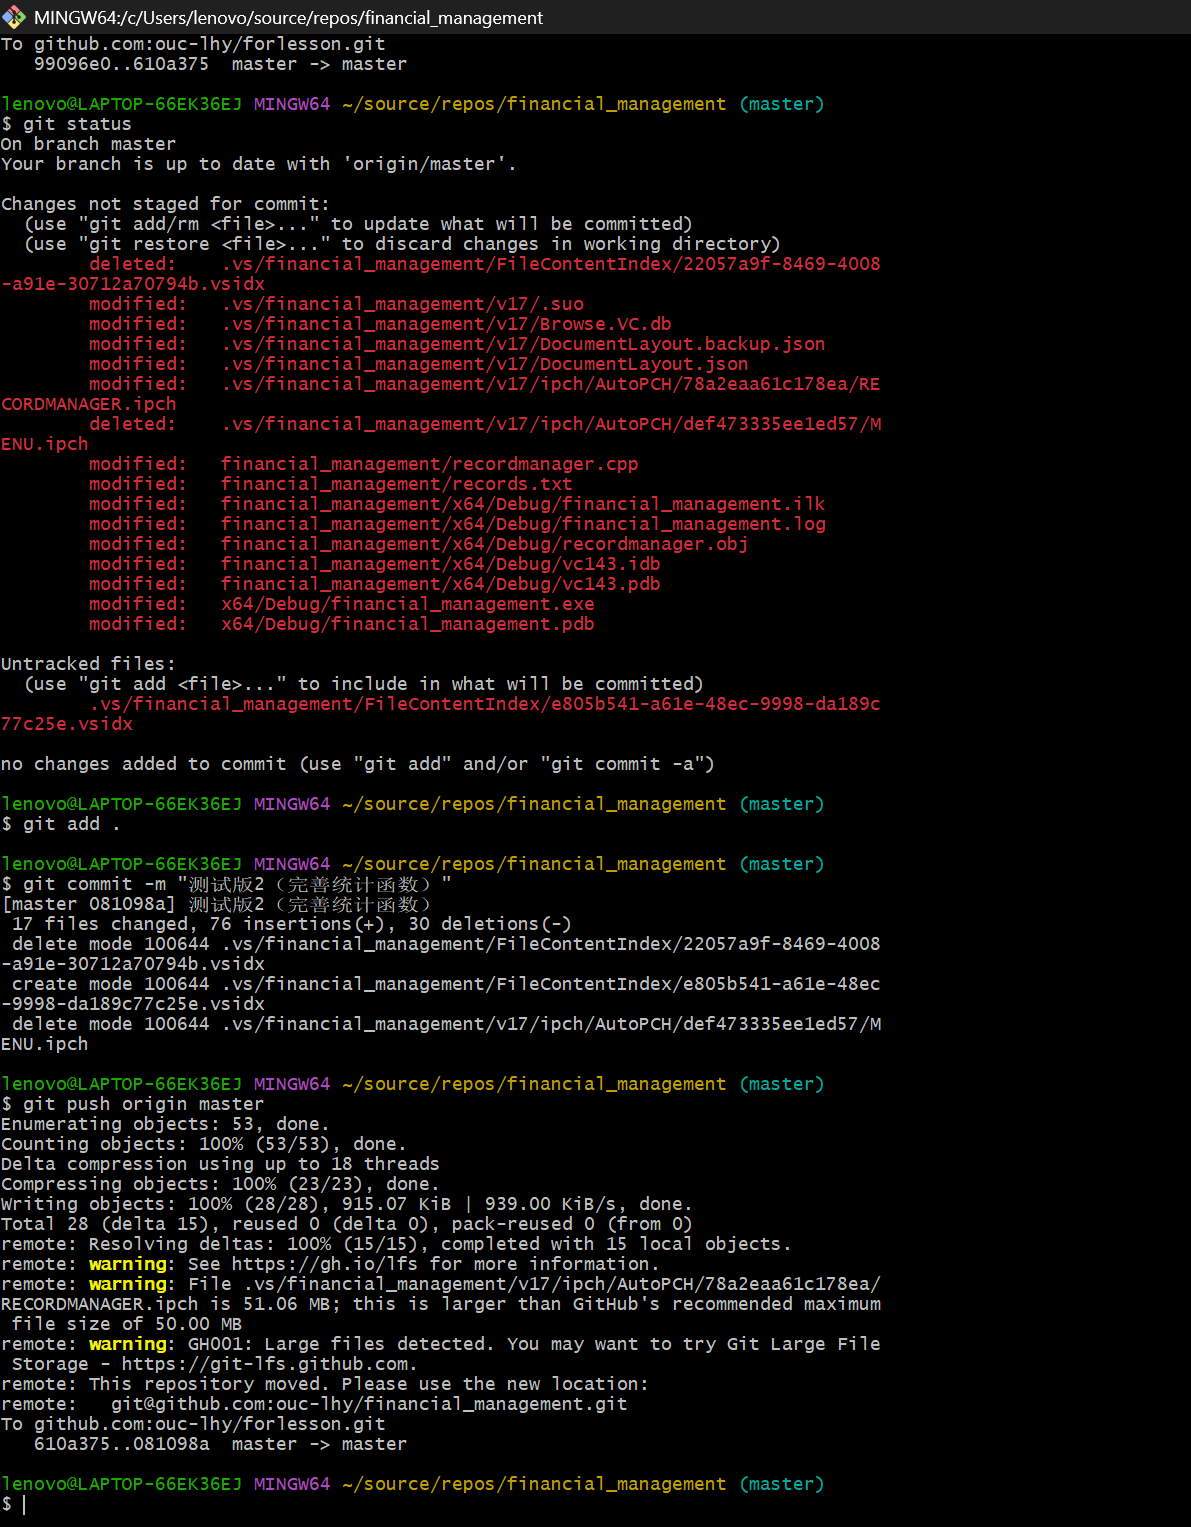
\includegraphics[width=0.8\textwidth]{git (1).png}
        \vspace{0.3cm} % 图片间的垂直间距
        \caption{Git 操作实例截图1}
        \label{fig:git-screenshot1}
    \end{figure}

    \begin{figure}[htbp]
        \centering
        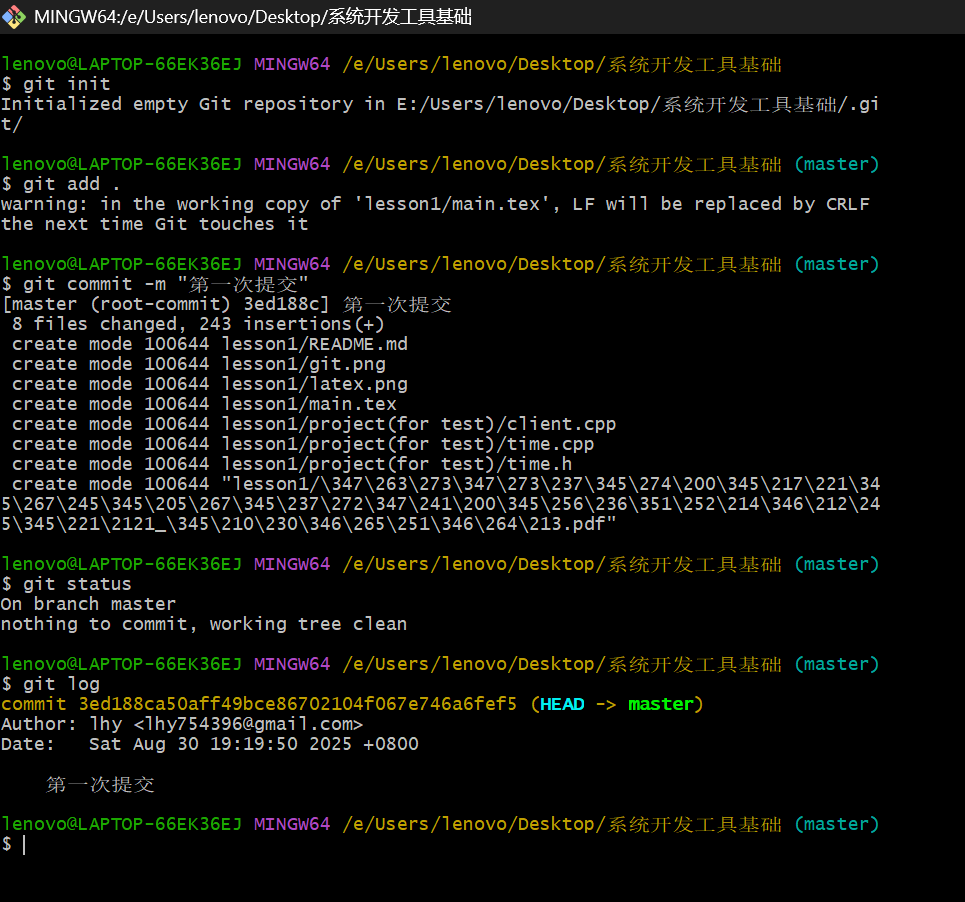
\includegraphics[width=0.8\textwidth]{git (2).png}
        \vspace{0.3cm} % 图片间的垂直间距
        \caption{Git 操作实例截图2}
        \label{fig:git-screenshot2}
    \end{figure}

    \begin{figure}[htbp]
        \centering
        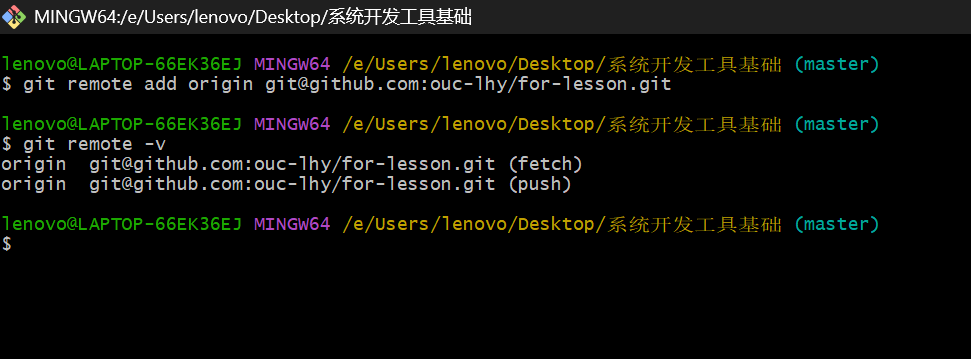
\includegraphics[width=0.8\textwidth]{git (3).png}
        \vspace{0.3cm} % 图片间的垂直间距
        \caption{Git 操作实例截图3}
        \label{fig:git-screenshot3}
    \end{figure}

    \begin{figure}[htbp]
        \centering
        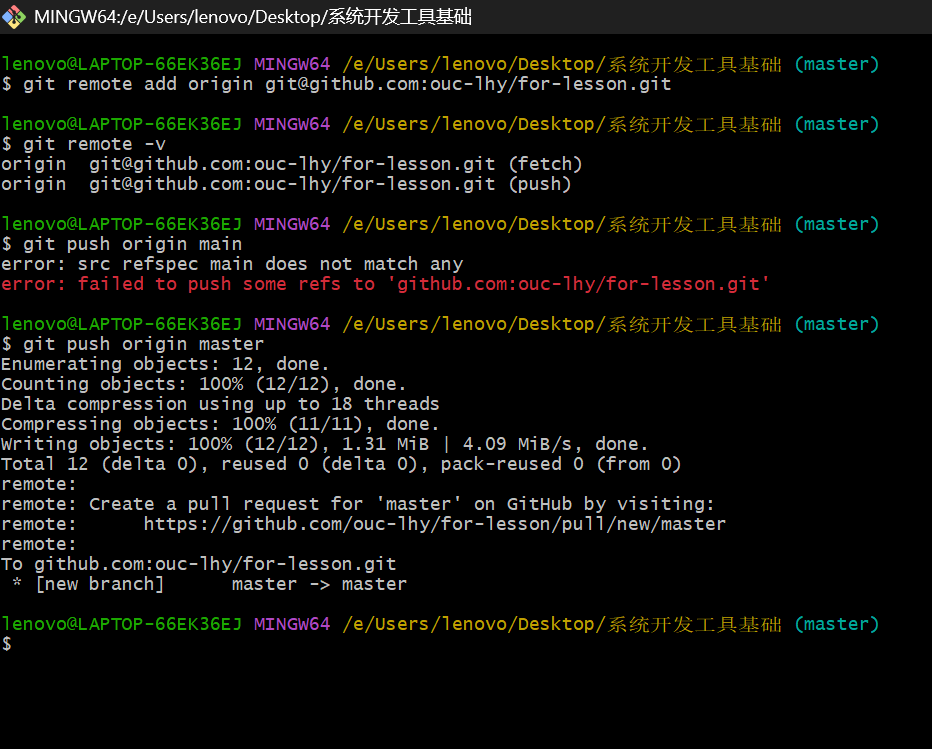
\includegraphics[width=0.8\textwidth]{git (4).png}
        \vspace{0.3cm} % 图片间的垂直间距
        \caption{Git 操作实例截图4}
        \label{fig:git-screenshot4}
    \end{figure}

    \begin{figure}[htbp]
        \centering
        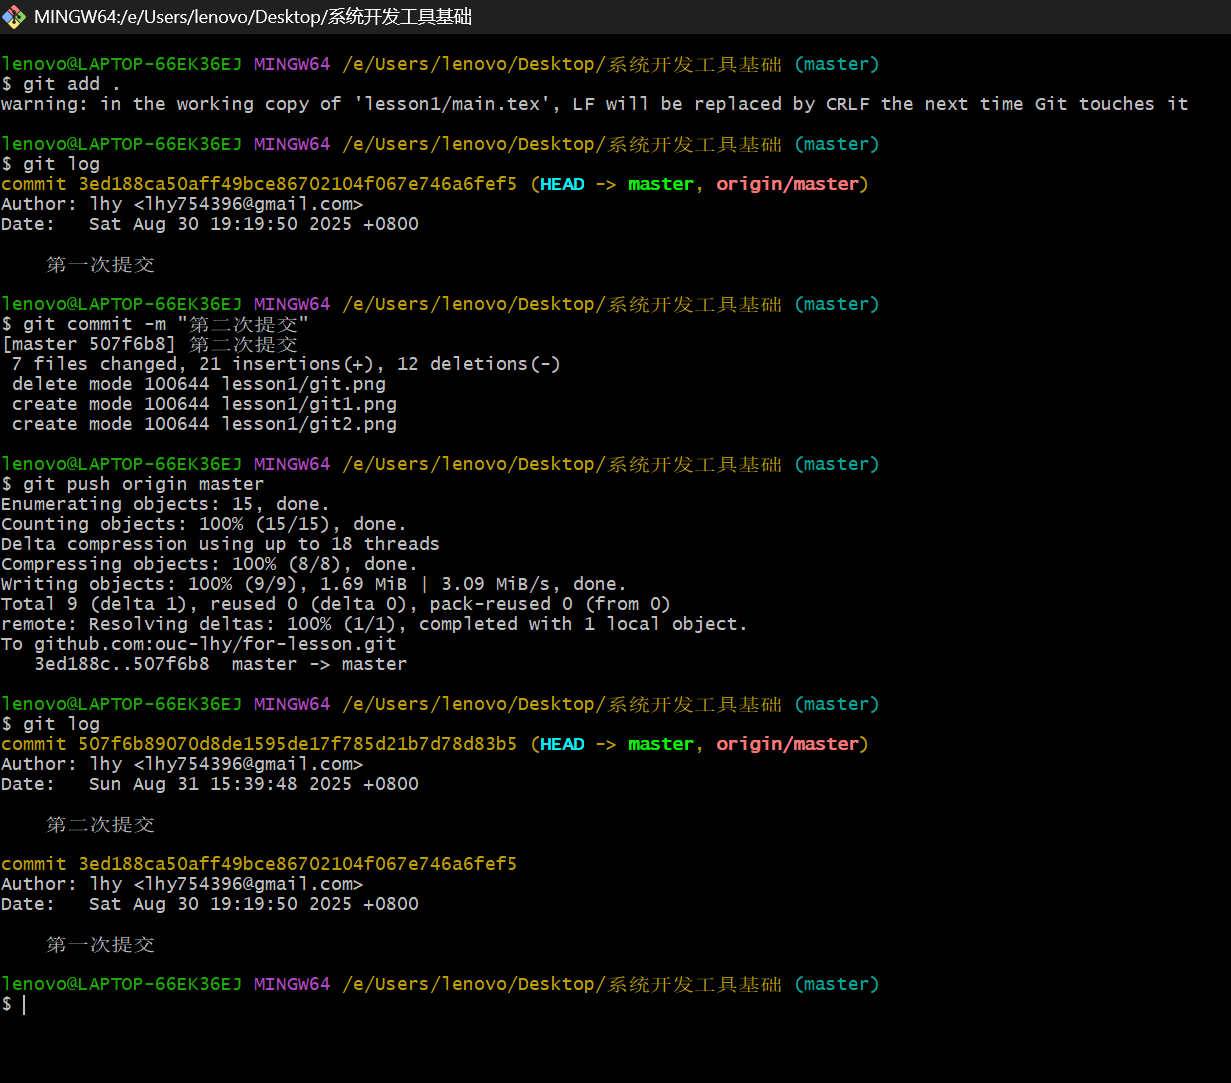
\includegraphics[width=0.8\textwidth]{git (5).png}
        \vspace{0.3cm} % 图片间的垂直间距
        \caption{Git 操作实例截图5}
        \label{fig:git-screenshot5}
    \end{figure}

    \begin{figure}[htbp]
        \centering
        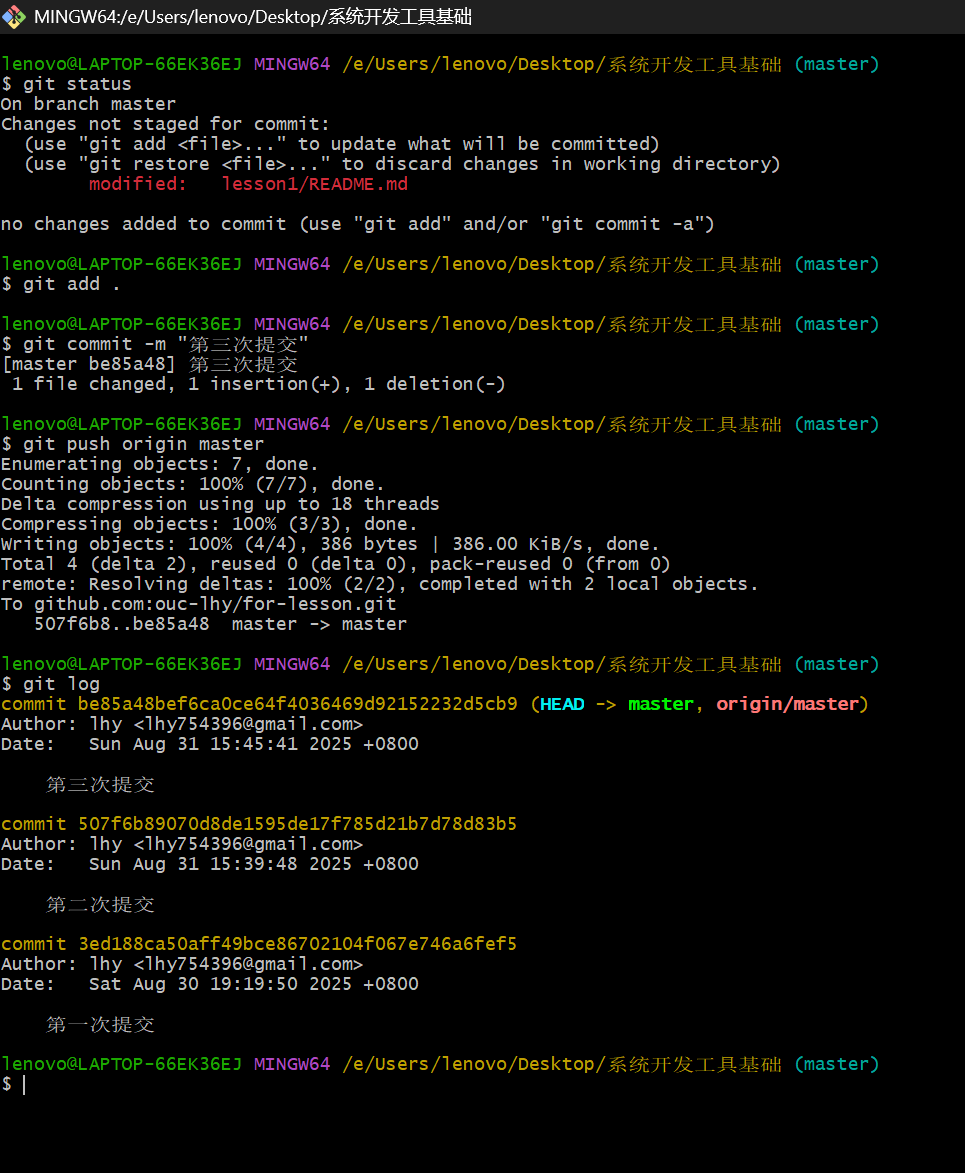
\includegraphics[width=0.8\textwidth]{git (6).png}
        \vspace{0.3cm} % 图片间的垂直间距
        \caption{Git 操作实例截图6}
        \label{fig:git-screenshot6}
    \end{figure}
    
\end{enumerate}


\begin{enumerate}
    \setcounter{enumi}{10} % 将计数器设置为10,下一个item将是11
    \item \begin{tcolorbox}[instancestyle]
        \textbf{实例11:文档结构} \\
        一个标准的LaTeX文档由文档类声明和文档环境组成。\\
        \texttt{\textbackslash documentclass\{article\}} 定义文档类型(如 article, report, book)。\\
        \texttt{\textbackslash begin\{document\}} 和 \texttt{\textbackslash end\{document\}} 标记正文开始和结束。\\
        所有正文内容必须位于这对命令之间。\\
        导言区(preamble)位于 \texttt{\textbackslash documentclass} 和 \texttt{\textbackslash begin\{document\}} 之间,用于加载宏包和设置全局选项。\\
        示例结构:
        \begin{verbatim}
        \documentclass{article}
        % 导言区:加载宏包、设置参数
        \usepackage{ctex}
        \begin{document}
        % 正文内容
        Hello, LaTeX!
        \end{document}
        \end{verbatim}
        理解文档结构是编写任何LaTeX文档的基础。\\
        编译时,LaTeX会处理整个结构,生成PDF。
    \end{tcolorbox}

    \begin{figure}[htbp]
        \centering
        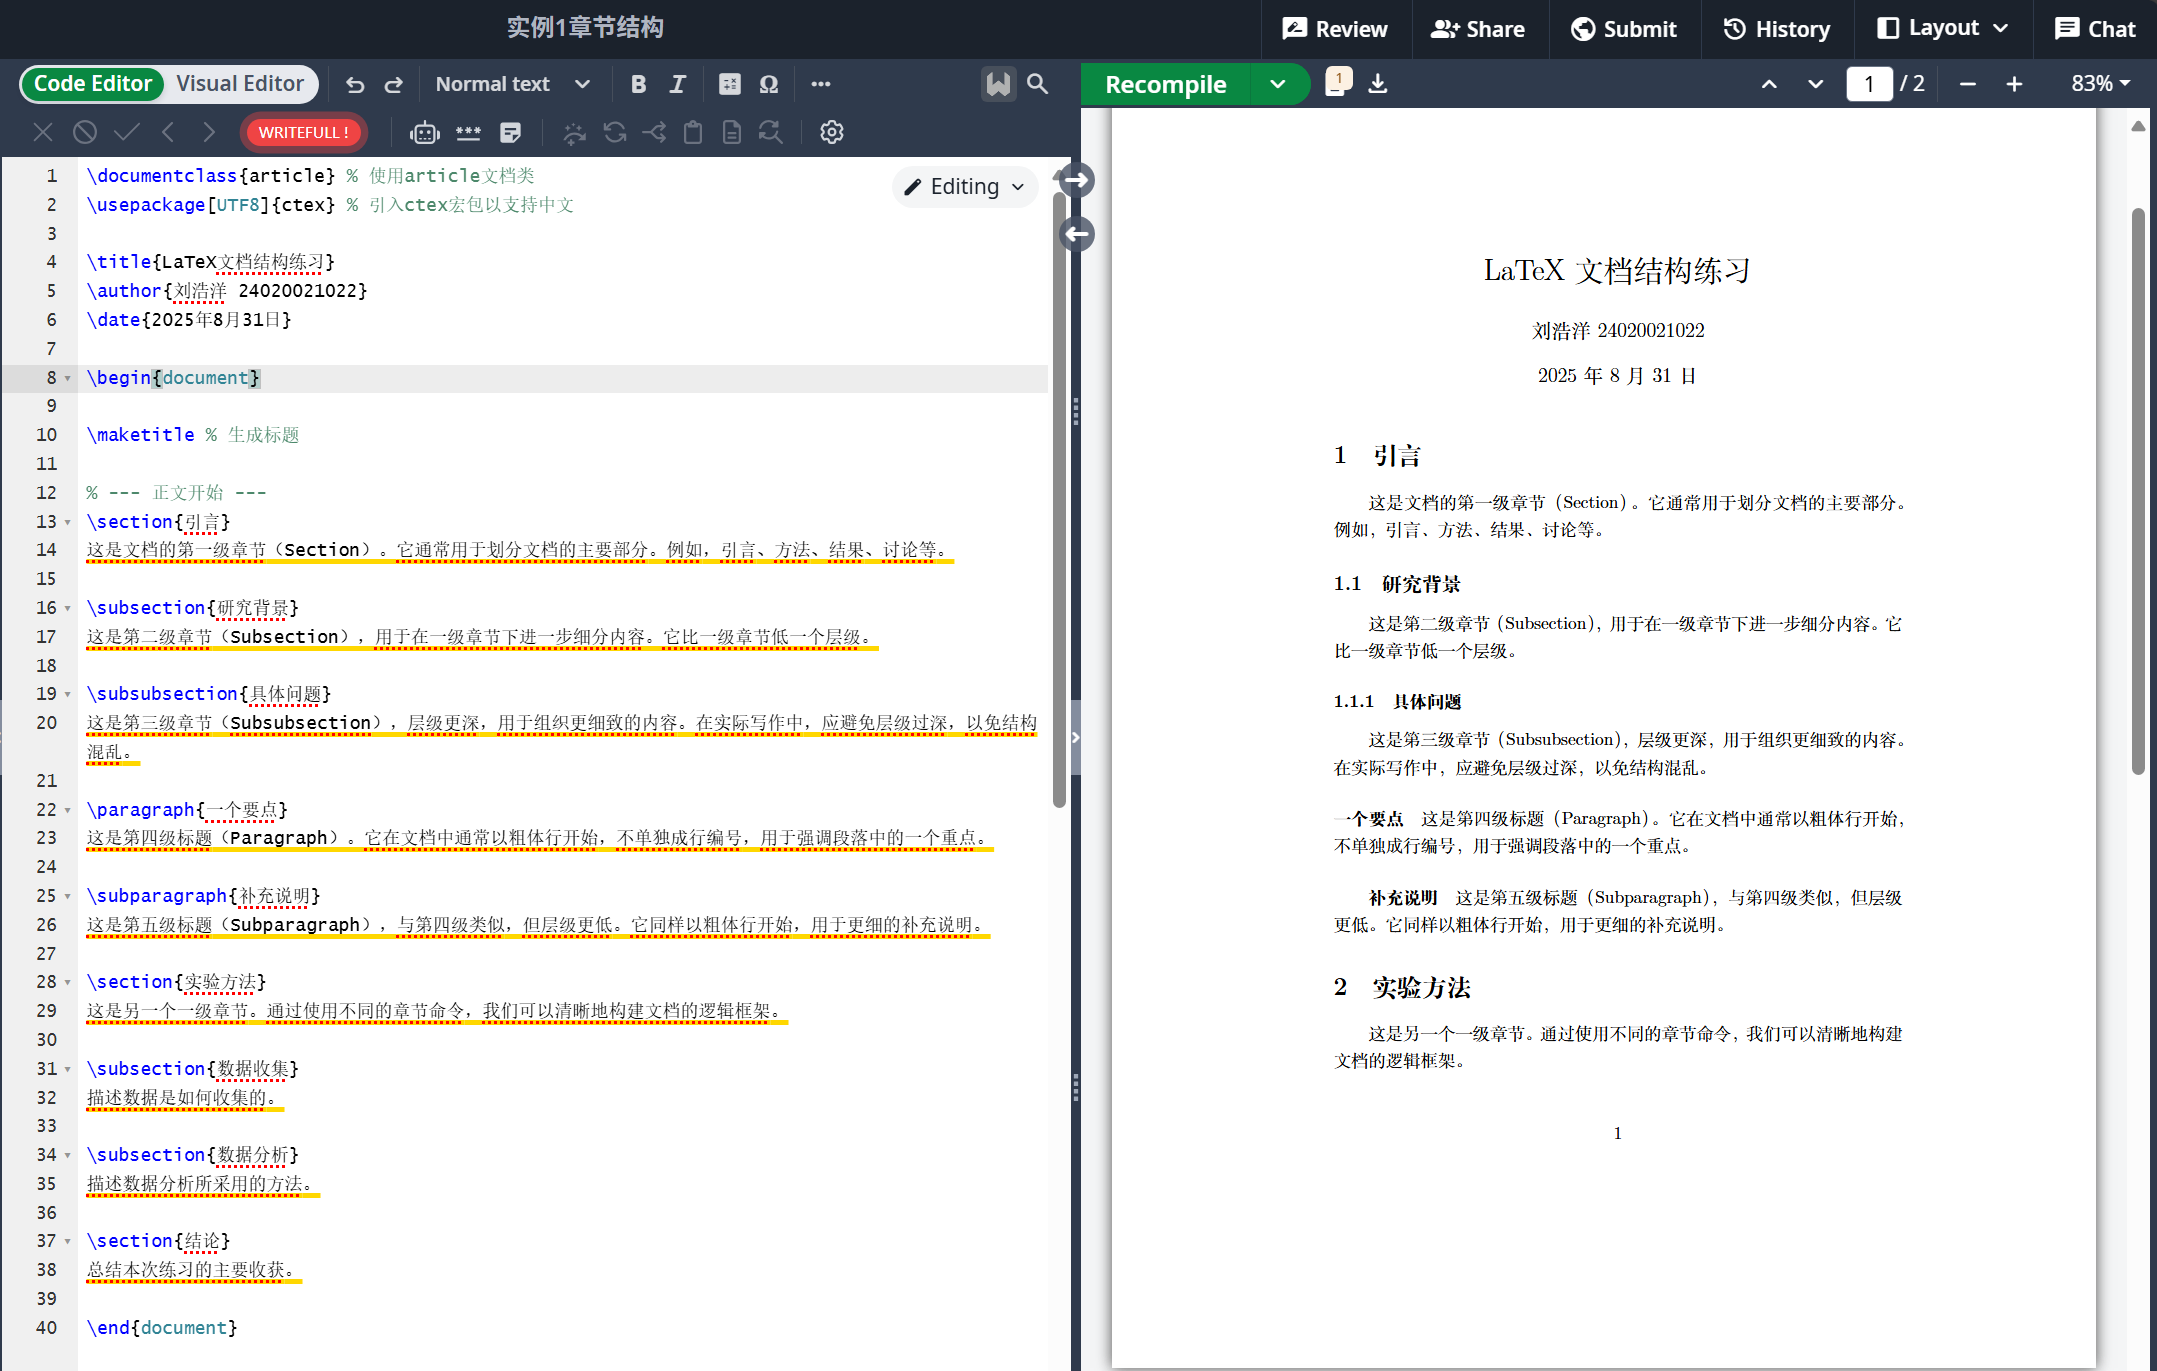
\includegraphics[width=0.8\textwidth]{latex 11.png}
        \caption{实例11:文档结构 示例截图}
        \label{fig:latex11}
    \end{figure}

    \item \begin{tcolorbox}[instancestyle]
        \textbf{实例12:章节与标题} \\
        \texttt{\textbackslash section\{...\}}, \texttt{\textbackslash subsection\{...\}}, \texttt{\textbackslash subsubsection\{...\}} 用于创建章节标题。\\
        操作:在文档正文中使用这些命令,如 \texttt{\textbackslash section\{引言\}}。\\
        效果:LaTeX会自动编号章节,并应用预设的标题格式(字体、大小、间距)。\\
        无编号章节:使用星号版本,如 \texttt{\textbackslash section*\{致谢\}}。\\
        应用场景:组织文档大纲,使结构清晰。\\
        \texttt{\textbackslash chapter\{...\}} 用于 book 和 report 类。\\
        章节命令会自动处理分页和间距,确保排版美观。\\
        可以在章节标题中使用数学公式或特殊字符。\\
        合理的章节划分是长文档可读性的关键。
    \end{tcolorbox}

    \item \begin{tcolorbox}[instancestyle]
        \textbf{实例13:文本格式化} \\
        LaTeX提供了多种命令来改变文本外观。\\
        \texttt{\textbackslash textbf\{粗体文本\}} 生成粗体。\\
        \texttt{\textbackslash textit\{斜体文本\}} 生成斜体。\\
        \texttt{\textbackslash underline\{下划线文本\}} 添加下划线。\\
        \texttt{\textbackslash emph\{强调\}} 通常为斜体,嵌套时行为更智能。\\
        作用:突出重点、表示变量名、书名等。\\
        注意:这些命令的参数是花括号 \{\} 内的文本。\\
        示例:\texttt{The variable \textbackslash textit\{x\} is important.} \\
        避免过度使用格式化,以免影响可读性。\\
        是日常文档编写中最常用的排版命令。
    \end{tcolorbox}

    \begin{figure}[htbp]
        \centering
        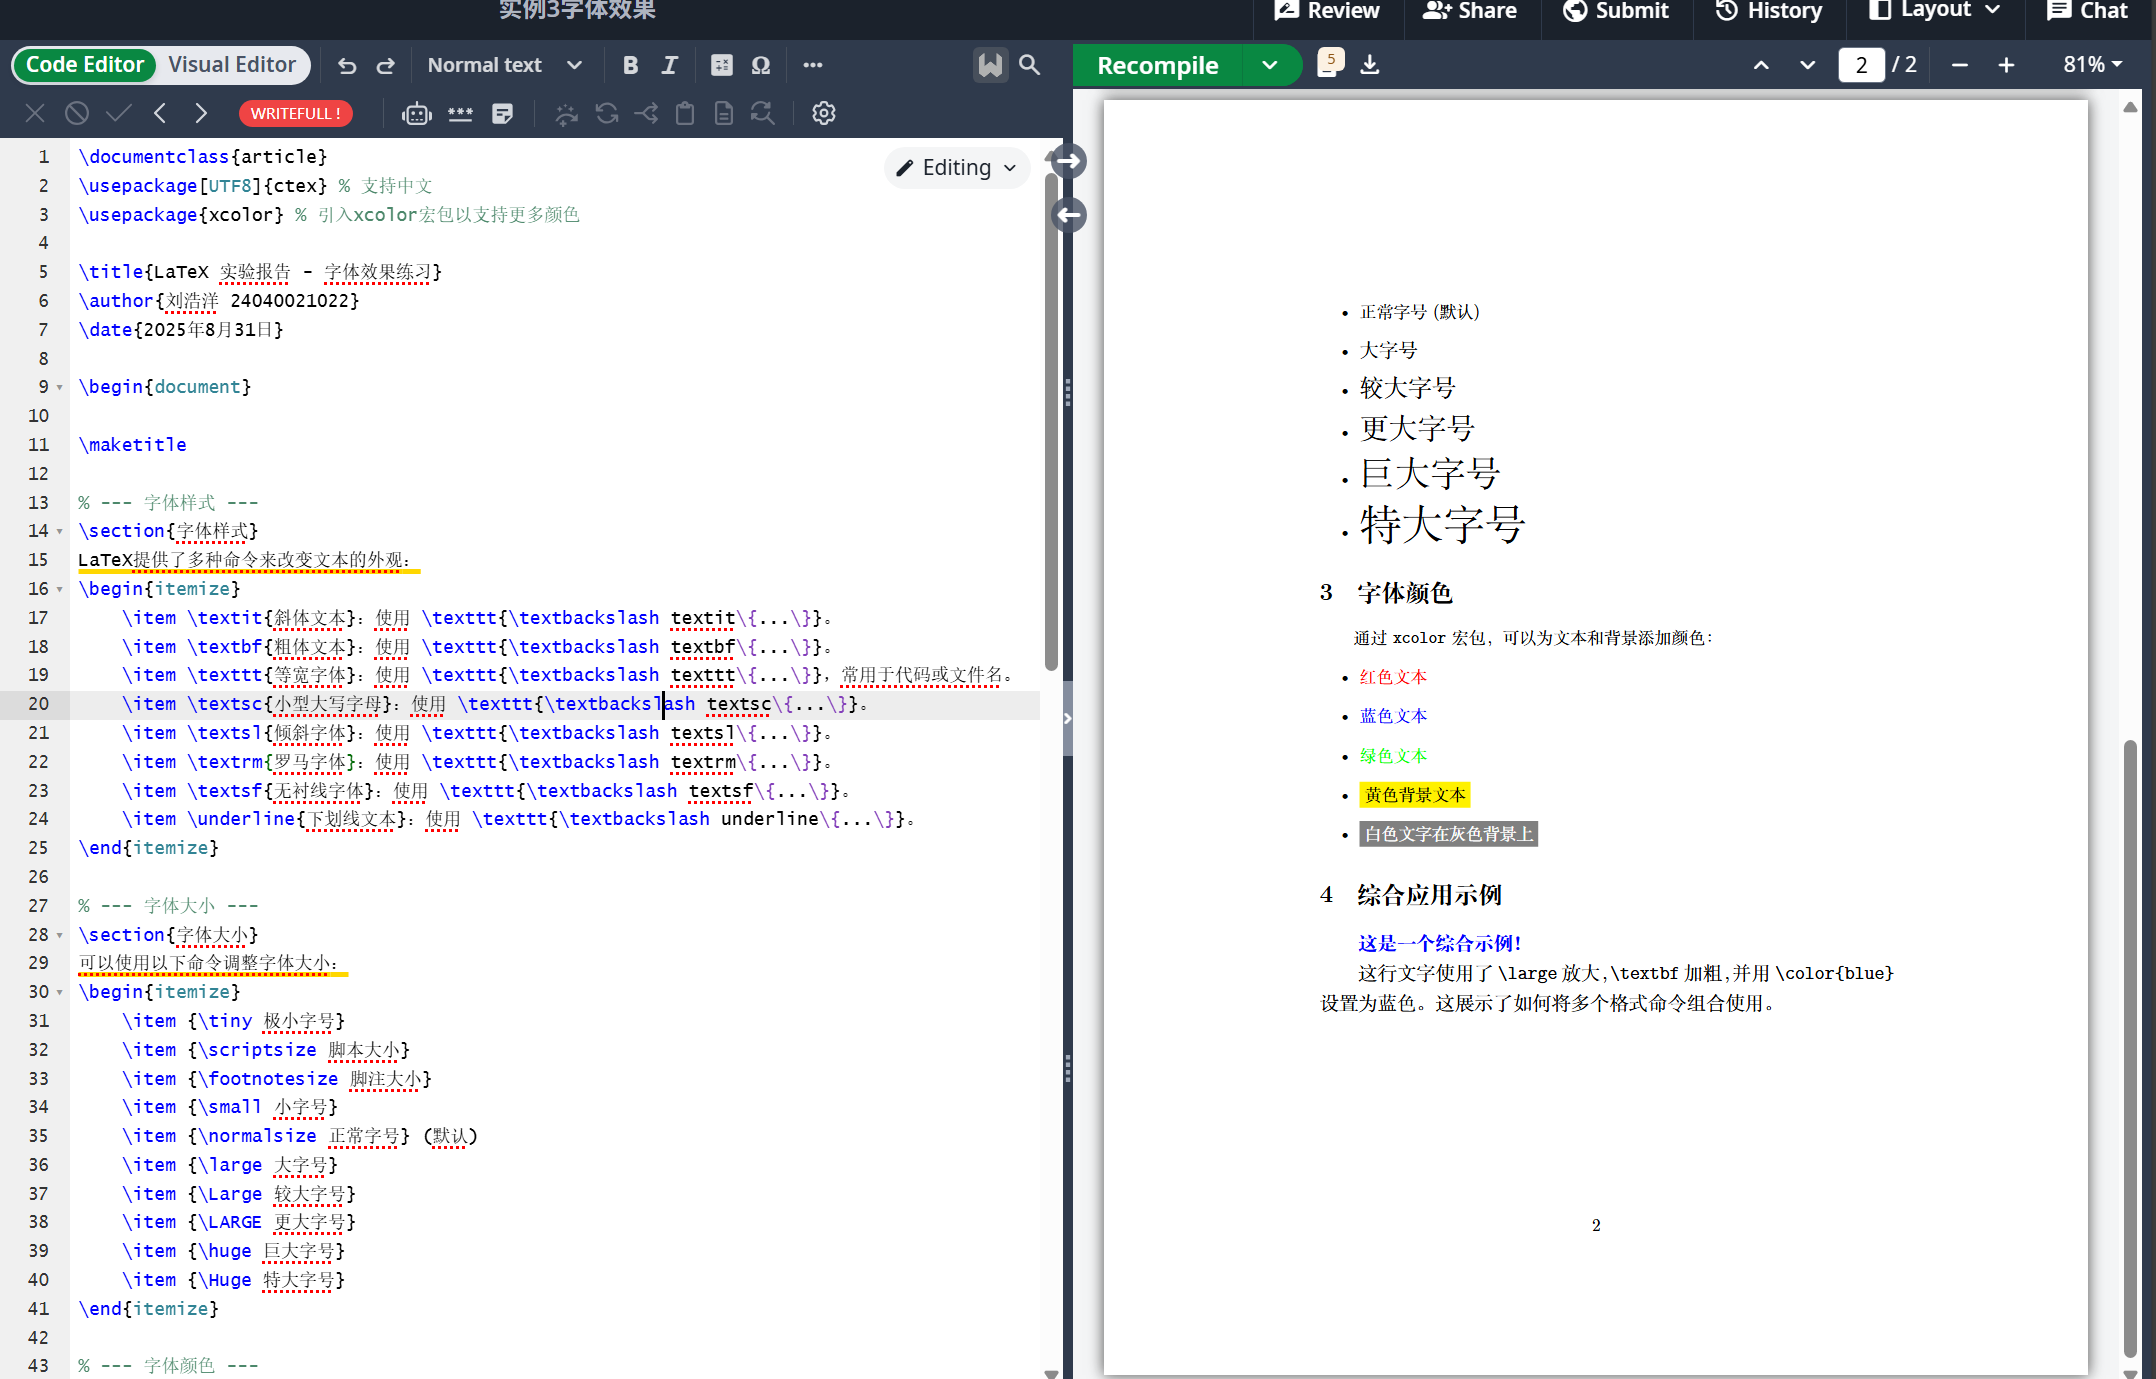
\includegraphics[width=0.8\textwidth]{latex 13.png}
        \caption{实例13:文本格式化 效果截图}
        \label{fig:latex13}
    \end{figure}

    \item \begin{tcolorbox}[instancestyle]
        \textbf{实例14:列表环境} \\
        LaTeX使用环境来创建列表。\\
        无序列表:\texttt{itemize} 环境,用 \texttt{\textbackslash item} 标记每项。\\
        有序列表:\texttt{enumerate} 环境,自动编号。\\
        示例:
        \begin{verbatim}
        \begin{itemize}
            \item 第一项
            \item 第二项
        \end{itemize}
        \end{verbatim}
        可以嵌套列表,创建多级结构。\\
        作用:清晰地罗列要点、步骤或项目。\\
        列表项可以包含多行文本、公式或图片。\\
        是制作提纲、任务列表和说明文档的理想选择。\\
        保持列表项简洁明了,增强可读性。
    \end{tcolorbox}

    \begin{figure}[htbp]
        \centering
        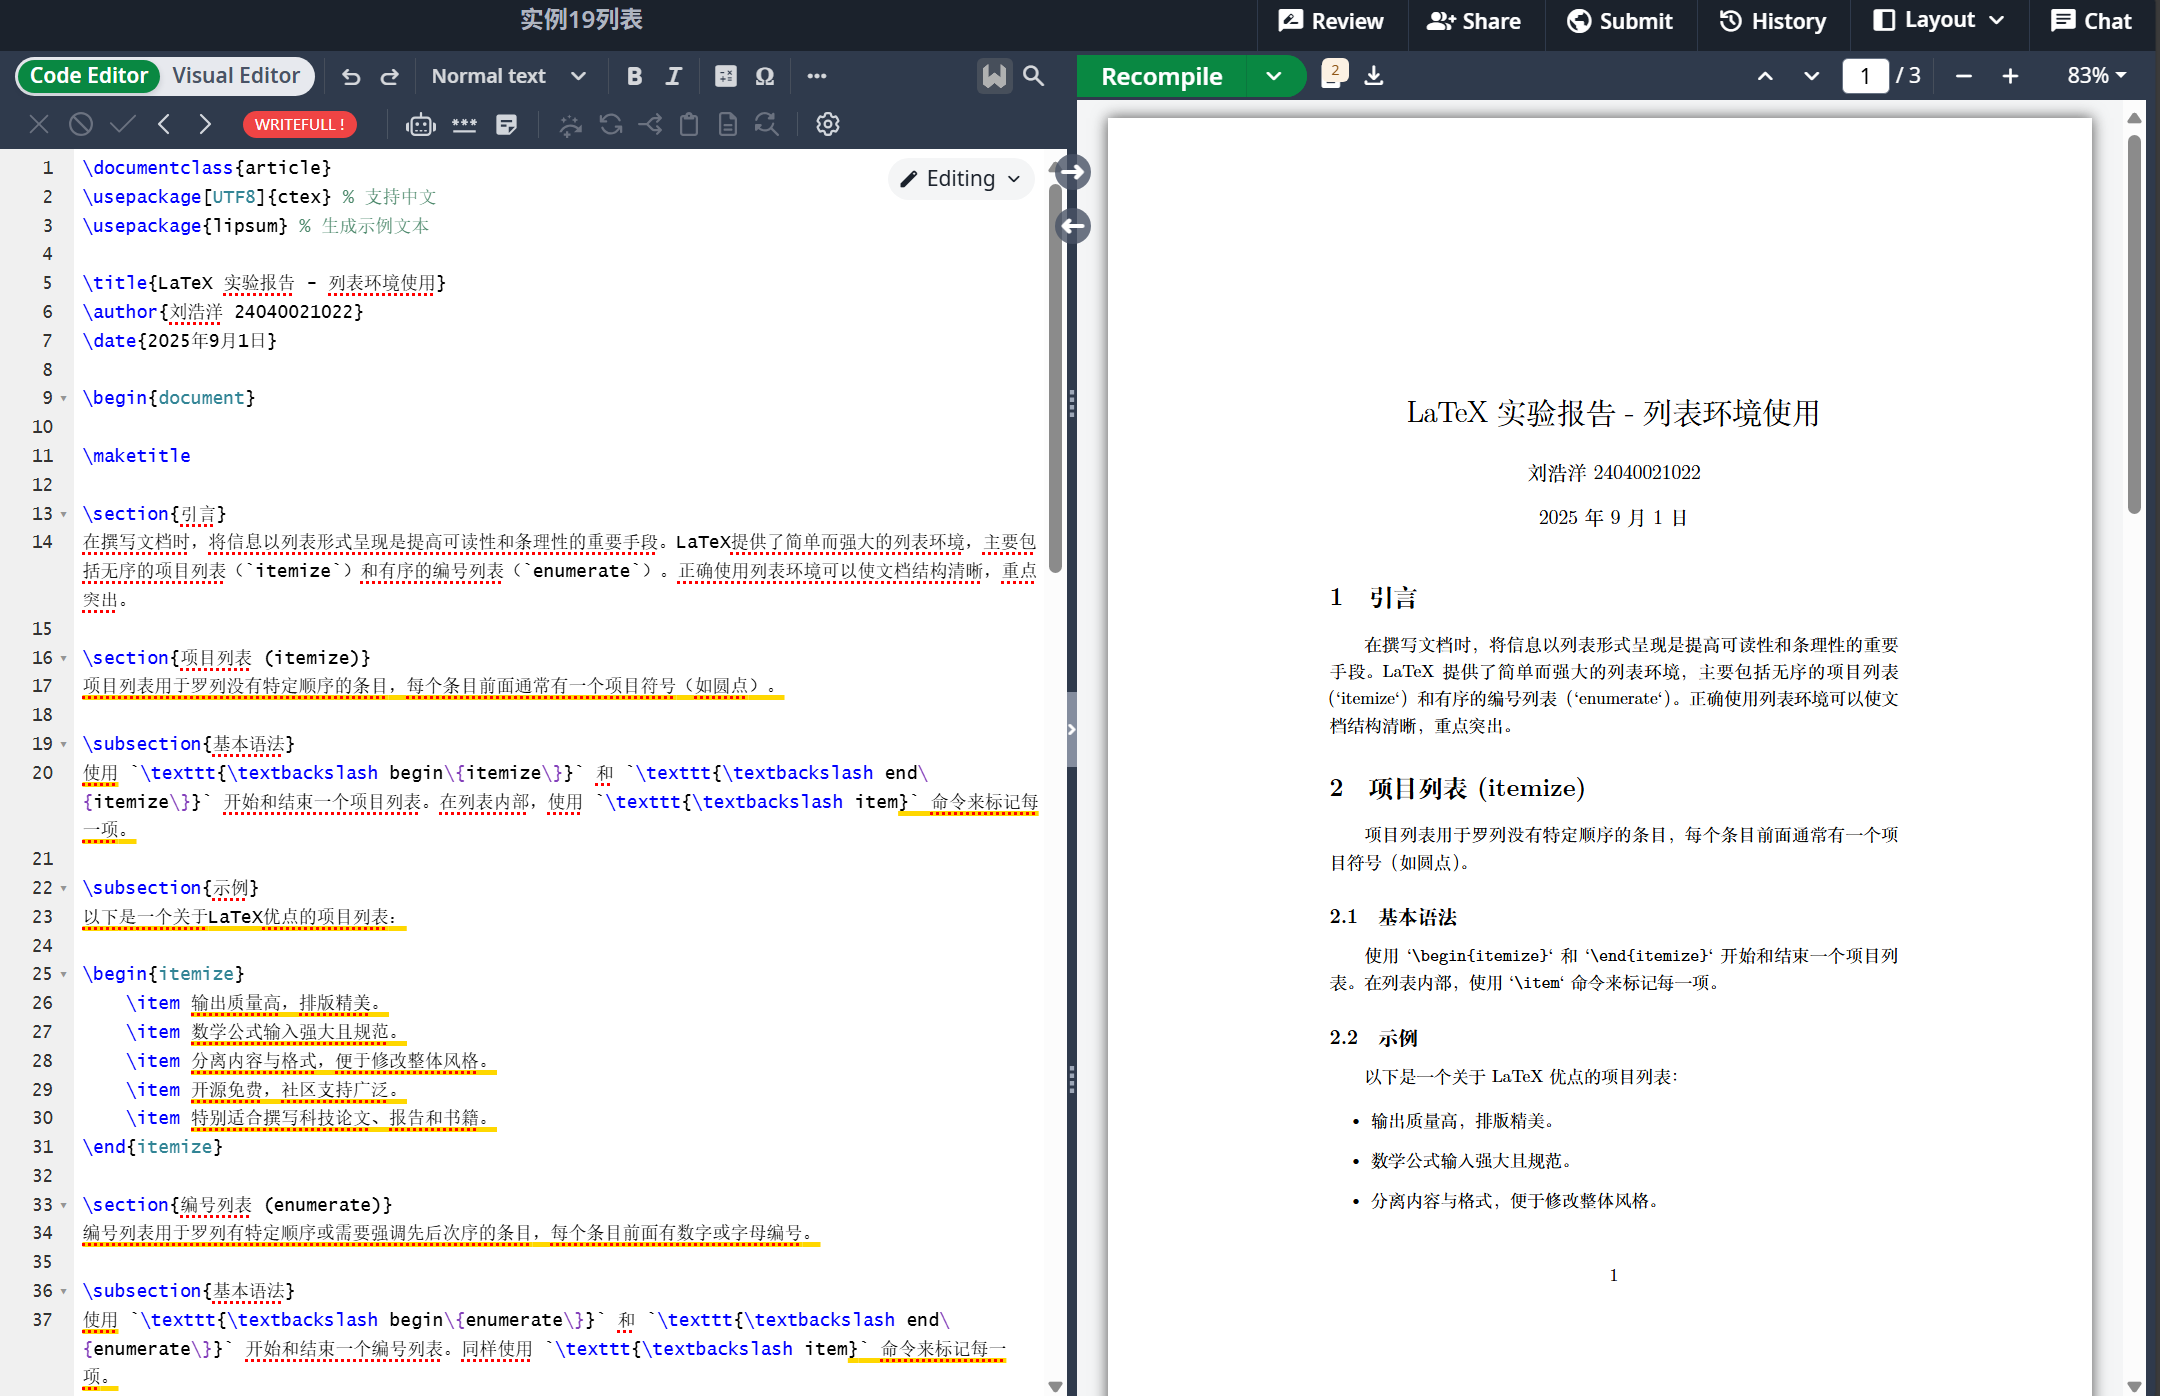
\includegraphics[width=0.8\textwidth]{latex 14.png}
        \caption{实例14:列表环境 效果截图}
        \label{fig:latex14}
    \end{figure}

    \item \begin{tcolorbox}[instancestyle]
        \textbf{实例15:插入图片} \\
        使用 \texttt{graphicx} 宏包和 \texttt{\textbackslash includegraphics} 命令插入图片。\\
        操作:先在导言区 \texttt{\textbackslash usepackage\{graphicx\}},然后在正文中使用命令。\\
        示例:\texttt{\textbackslash includegraphics[width=0.5\textbackslash textwidth]\{image.png\}}。\\
        参数:\texttt{width}, \texttt{height}, \texttt{scale} 控制图片大小。\\
        通常将图片放入 \texttt{figure} 浮动环境,以便自动排版和添加标题。\\
        使用 \texttt{\textbackslash caption\{...\}} 添加图注,\texttt{\textbackslash label\{...\}} 添加标签以便引用。\\
        支持多种格式:PNG, JPG, PDF(推荐矢量图)。\\
        图片路径可以是相对路径或绝对路径。\\
        是制作报告、论文不可或缺的功能。
    \end{tcolorbox}

    \begin{figure}[htbp]
        \centering
        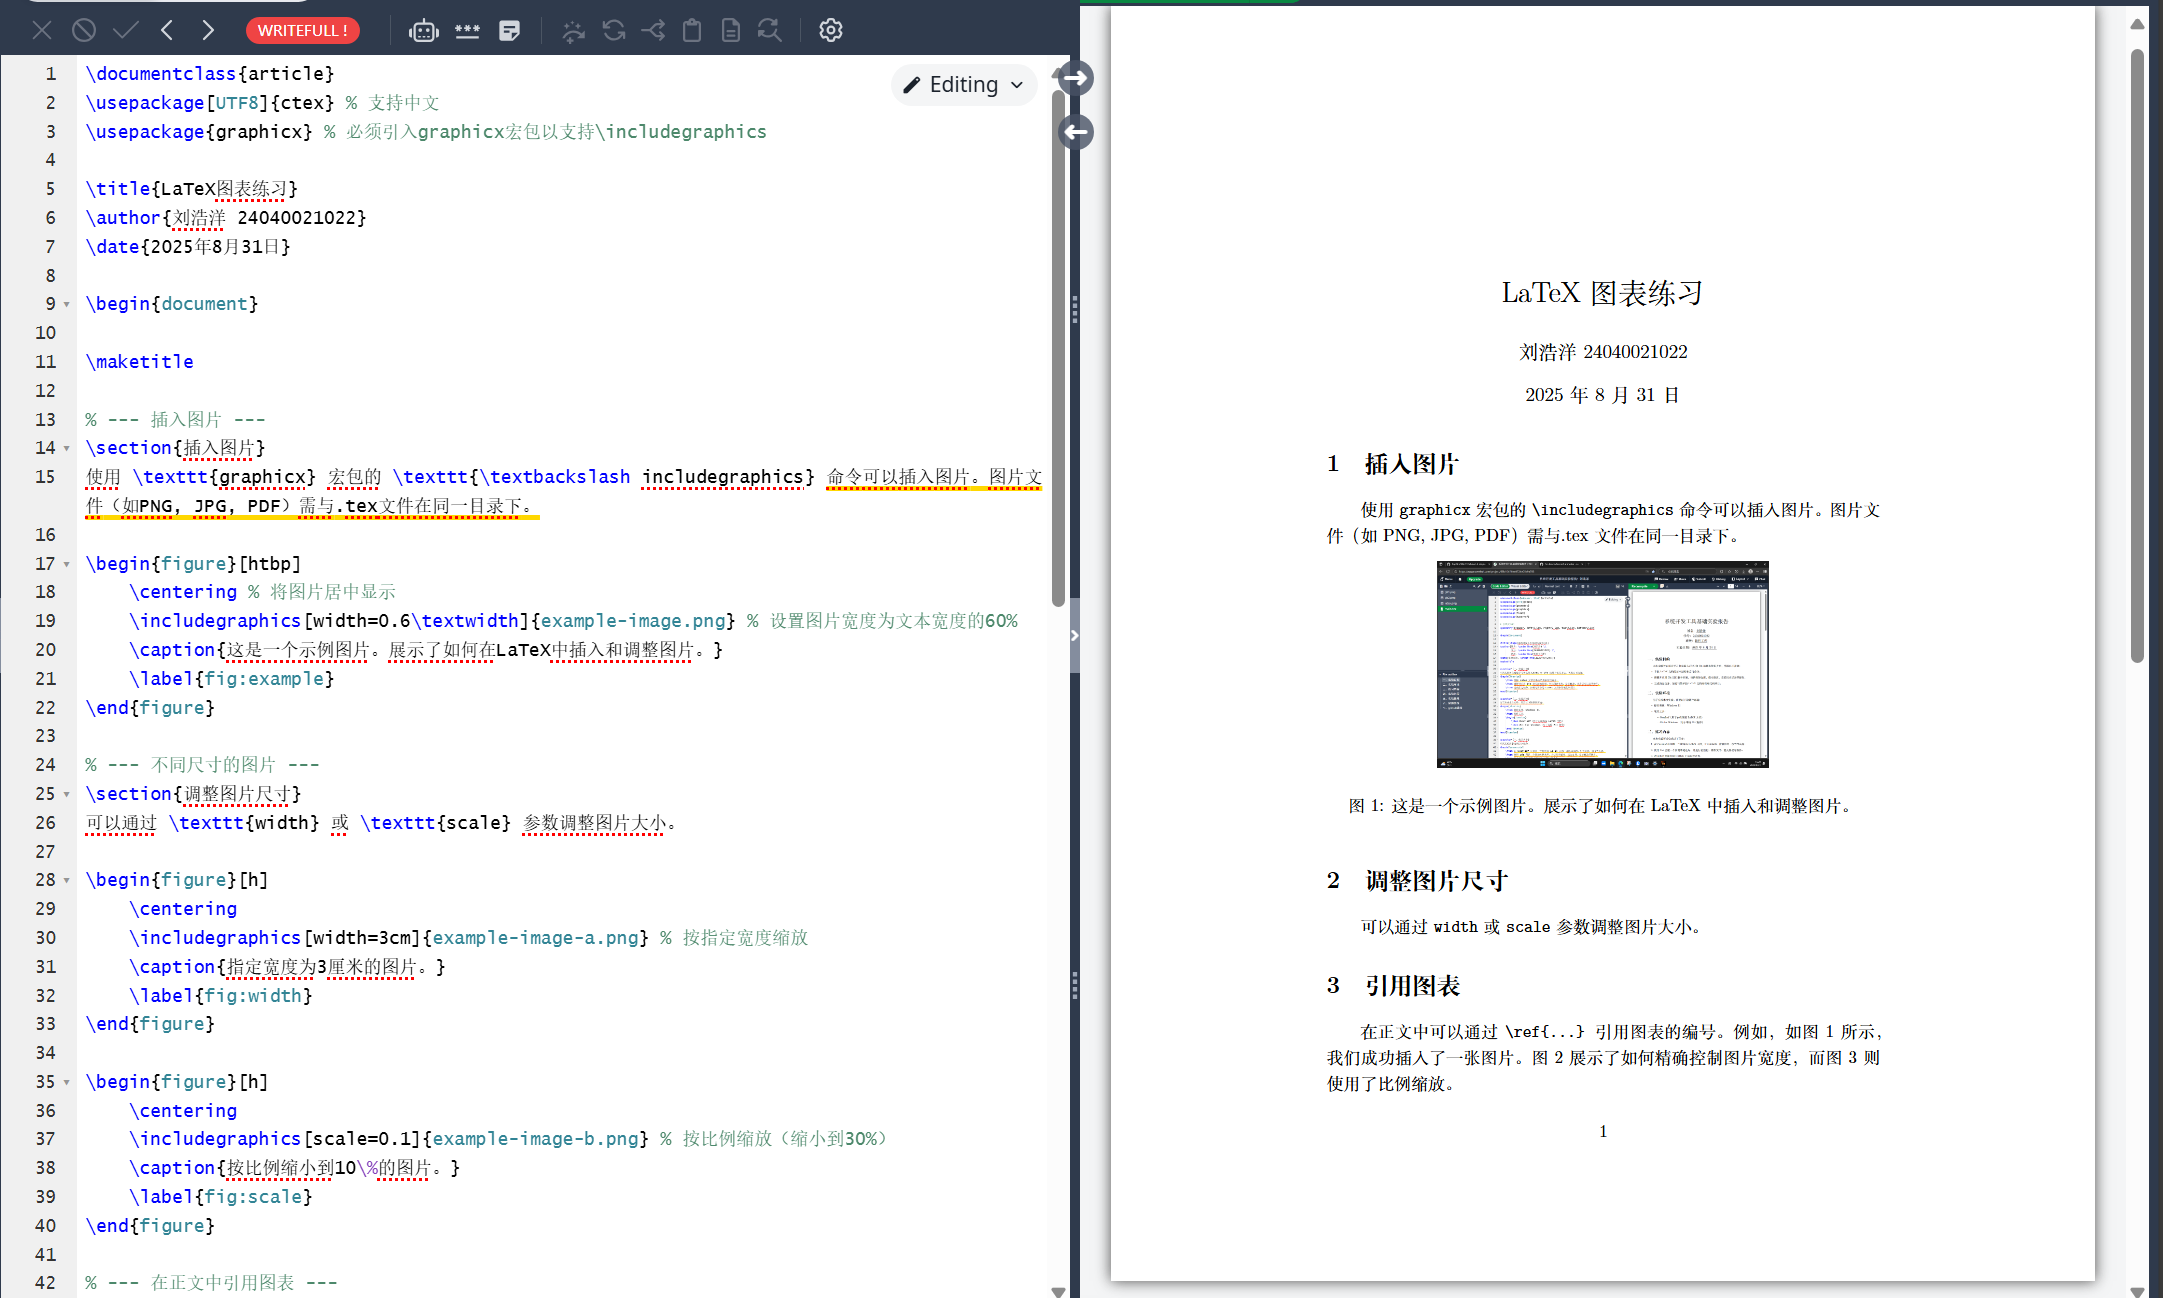
\includegraphics[width=0.8\textwidth]{latex 15.png}
        \caption{实例15:插入图片 操作截图}
        \label{fig:latex15}
    \end{figure}

    \item \begin{tcolorbox}[instancestyle]
        \textbf{实例16:创建表格} \\
        使用 \texttt{tabular} 环境创建表格。\\
        语法:\texttt{\textbackslash begin\{tabular\}\{lcr|\}},其中 l,c,r 表示左、中、右对齐,| 表示竖线。\\
        行内分隔:用 \& 分隔列,用 \textbackslash\textbackslash 换行。\\
        示例:
        \begin{verbatim}
        \begin{tabular}{|l|c|r|}
        \hline
        左对齐 & 居中 & 右对齐 \\ \hline
        A & B & C \\ \hline
        \end{tabular}
        \end{verbatim}
        \texttt{\textbackslash hline} 添加横线。\\
        可放入 \texttt{table} 浮动环境,添加表标题和标签。\\
        复杂表格可使用 \texttt{booktabs} 宏包获得更专业的外观。\\
        是展示数据和对比信息的有效方式。
    \end{tcolorbox}

    \item \begin{tcolorbox}[instancestyle]
    \textbf{实例17:数学公式} \\
    LaTeX是排版数学公式的黄金标准。\\
    行内公式:用 \texttt{\$...\$} 包围,如 \texttt{\$E=mc\^{}2\$},公式与文本同行。\\
    行间公式:用 \texttt{\textbackslash[...\textbackslash]} 或 \texttt{\textbackslash begin\{equation\}...\textbackslash end\{equation\}},公式单独成行并可编号。\\
    常用符号:\texttt{\textasciicircum} 上标,\texttt{\_} 下标,\texttt{\textbackslash frac\{a\}\{b\}} 分数,\texttt{\textbackslash sqrt\{x\}} 开方。\\
    示例:\texttt{\textbackslash[ \textbackslash int\_0\^{}\textbackslash infty e\^{}\{-x\^{}2\} dx = \textbackslash frac\{\textbackslash sqrt\{\textbackslash pi\}\}\{2\} \textbackslash]}。\\
    需要 \texttt{amsmath} 等宏包支持高级数学环境。\\
    公式可使用 \texttt{\textbackslash label} 和 \texttt{\textbackslash ref} 进行引用。\\
    是撰写科技论文的核心技能。
    \end{tcolorbox}

    \begin{figure}[htbp]
        \centering
        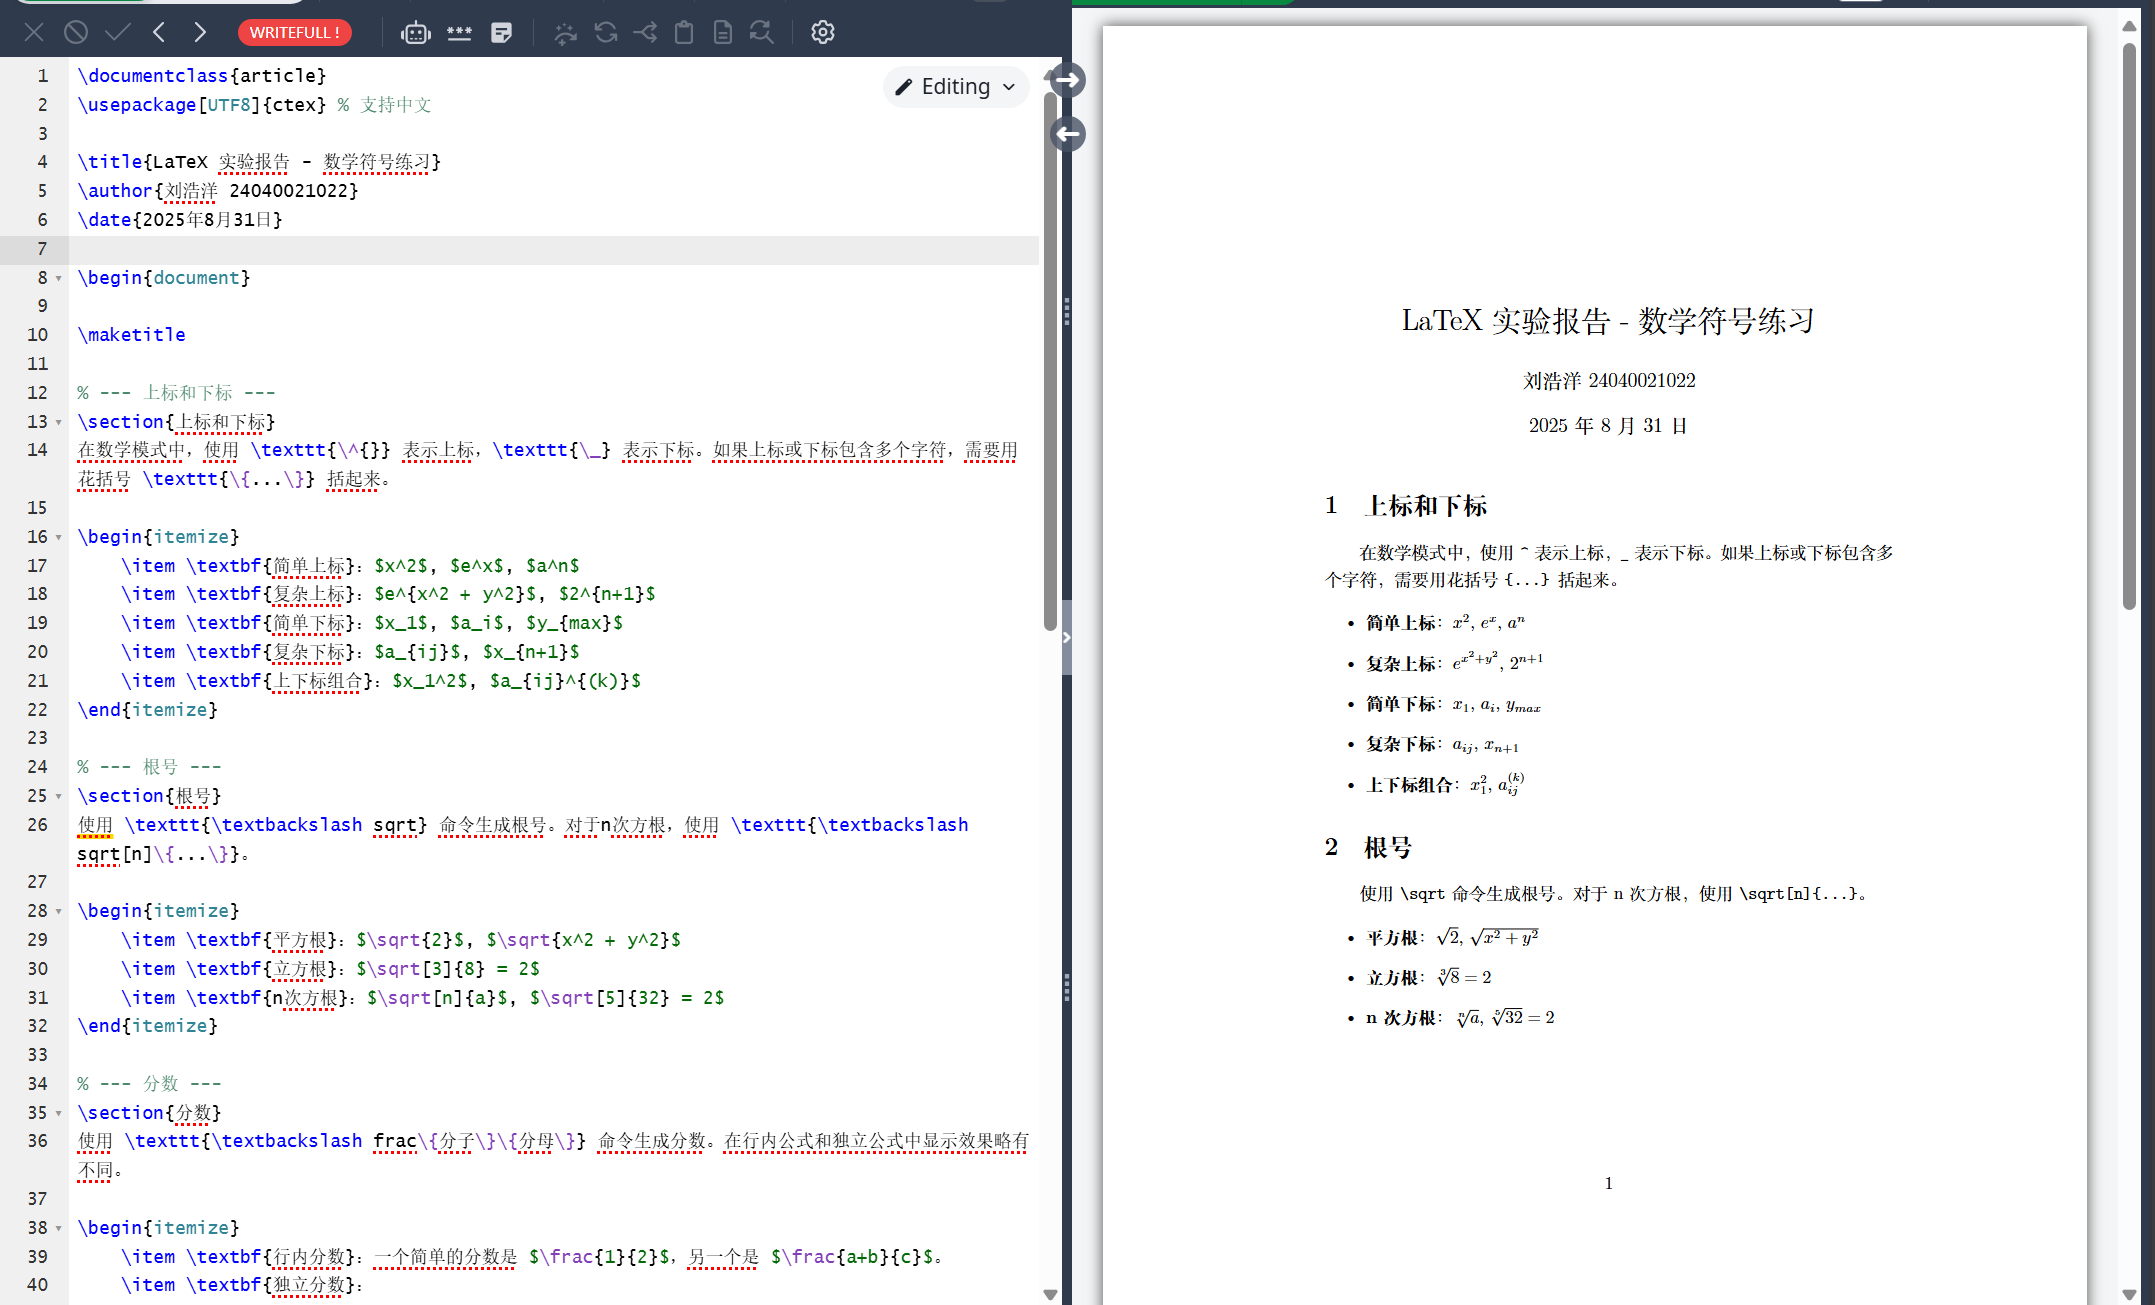
\includegraphics[width=0.8\textwidth]{latex 17.png}
        \caption{实例17:数学公式 排版效果截图}
        \label{fig:latex17}
    \end{figure}

    \item \begin{tcolorbox}[instancestyle]
        \textbf{实例18:超链接} \\
        使用 \texttt{hyperref} 宏包创建超链接。\\
        操作:在导言区 \texttt{\textbackslash usepackage\{hyperref\}}。\\
        创建网页链接:\texttt{\textbackslash href\{https://example.com\}\{访问网站\}}。\\
        显示URL:\texttt{\textbackslash url\{https://example.com\}}。\\
        内部链接:\texttt{\textbackslash ref\{fig:myfig\}} 引用图片或表格,\texttt{\textbackslash pageref\{sec:intro\}} 引用页码。\\
        效果:生成的PDF中,链接可点击跳转。\\
        可自定义链接颜色等外观(可选)。\\
        极大提升了电子文档的交互性和可用性。\\
        是现代文档不可或缺的功能。
    \end{tcolorbox}

    \item \begin{tcolorbox}[instancestyle]
        \textbf{实例19:段落与缩进} \\
        LaTeX中,一个空行表示新段落的开始。\\
        首行缩进由 \texttt{\textbackslash parindent} 控制。\\
        操作:在导言区用 \texttt{\textbackslash setlength\{\textbackslash parindent\}\{2em\}} 设置缩进量(如2个汉字宽)。\\
        取消单个段落缩进:在段落开头使用 \texttt{\textbackslash noindent}。\\
        全局取消缩进:\texttt{\textbackslash setlength\{\textbackslash parindent\}\{0pt\}}。\\
        换行:在行末使用 \texttt{\textbackslash\textbackslash} 强制换行(不开始新段落)。\\
        分页:\texttt{\textbackslash newpage} 或 \texttt{\textbackslash clearpage}。\\
        合理的段落处理是中文排版的基本要求。\\
        确保段落间距和缩进符合文档规范。
    \end{tcolorbox}

    \item \begin{tcolorbox}[instancestyle]
    \textbf{实例20:函数图像} \\
    使用 \texttt{pgfplots} 宏包(基于 \texttt{tikz})绘制高质量函数图像。\\
    操作:在导言区 \texttt{\textbackslash usepackage\{pgfplots\}}, \texttt{\textbackslash pgfplotsset\{compat=1.18\}}。\\
    在正文中使用 \texttt{tikzpicture} 和 \texttt{axis} 环境。\\
    示例:绘制 $y=x^2$。
    \begin{verbatim}
    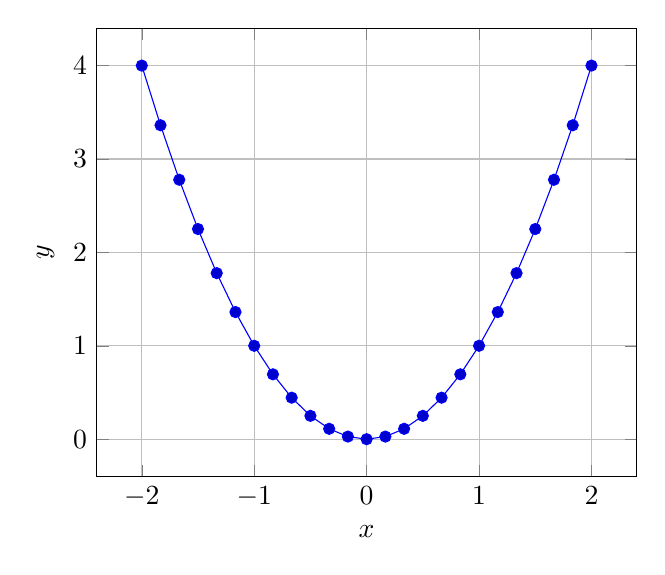
\begin{tikzpicture}
    \begin{axis}[
        xlabel=$x$, ylabel=$y$,
        grid=both, domain=-2:2
    ]
    \addplot {x^2};
    \end{axis}
    \end{tikzpicture}
    \end{verbatim}
    可绘制复杂函数、数据点、三维图等。\\
    支持精细的样式控制(线型、颜色、图例)。\\
    图像为矢量图,无限缩放不失真。\\
    是科技文档中展示数学关系的完美工具。
    \end{tcolorbox}

    \begin{figure}[htbp]
        \centering
        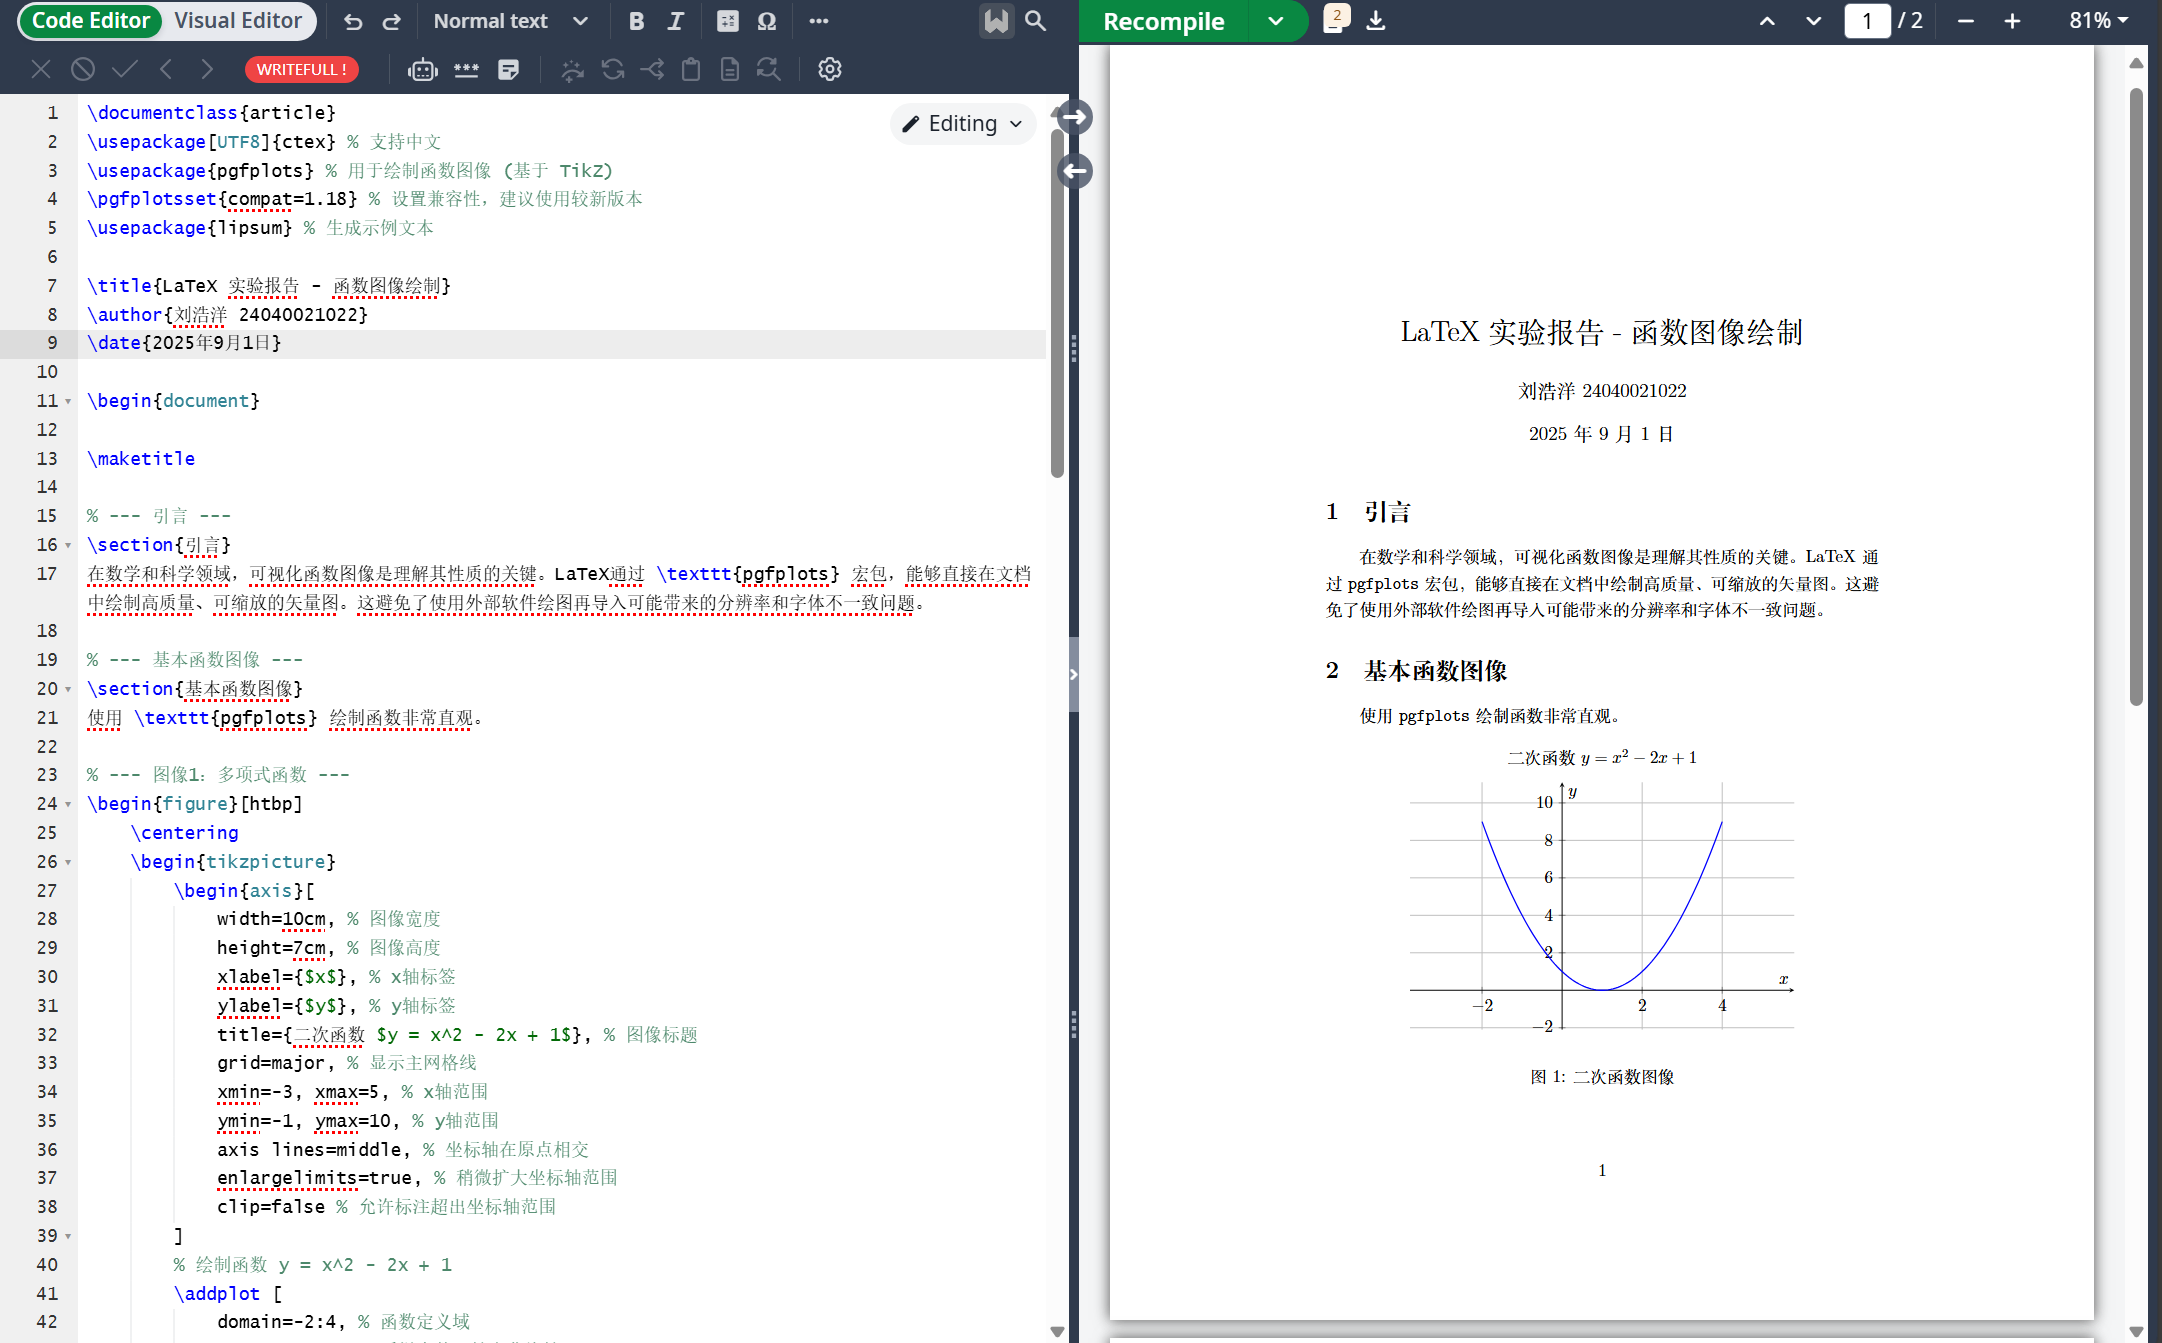
\includegraphics[width=0.8\textwidth]{latex 20.png}
        \caption{实例20:函数图像 绘制效果截图}
        \label{fig:latex20}
    \end{figure}
    
\end{enumerate}

\newpage
\section*{五、实验结果}
在本次实验中,成功完成了以下任务:
\begin{itemize}
    \item 系统地完成了20个实例,前10个了解了Git基础命令,后10个了解了LaTeX核心排版技能。
    \item 创建了一个结构完整、格式规范的LaTeX实验报告,实现了标题、作者信息、章节、列表、图片、公式、超链接等多种元素的集成。
    \item 使用 Git 进行了高效的版本控制,创建了本地仓库并进行了多次提交,完整记录了学习过程。
    \item 成功将项目推送到 GitHub 远程仓库:\url{https://github.com/ouc-lhy/for-lesson/tree/master/lesson1}
\end{itemize}

\begin{figure}[htbp]
        \centering
        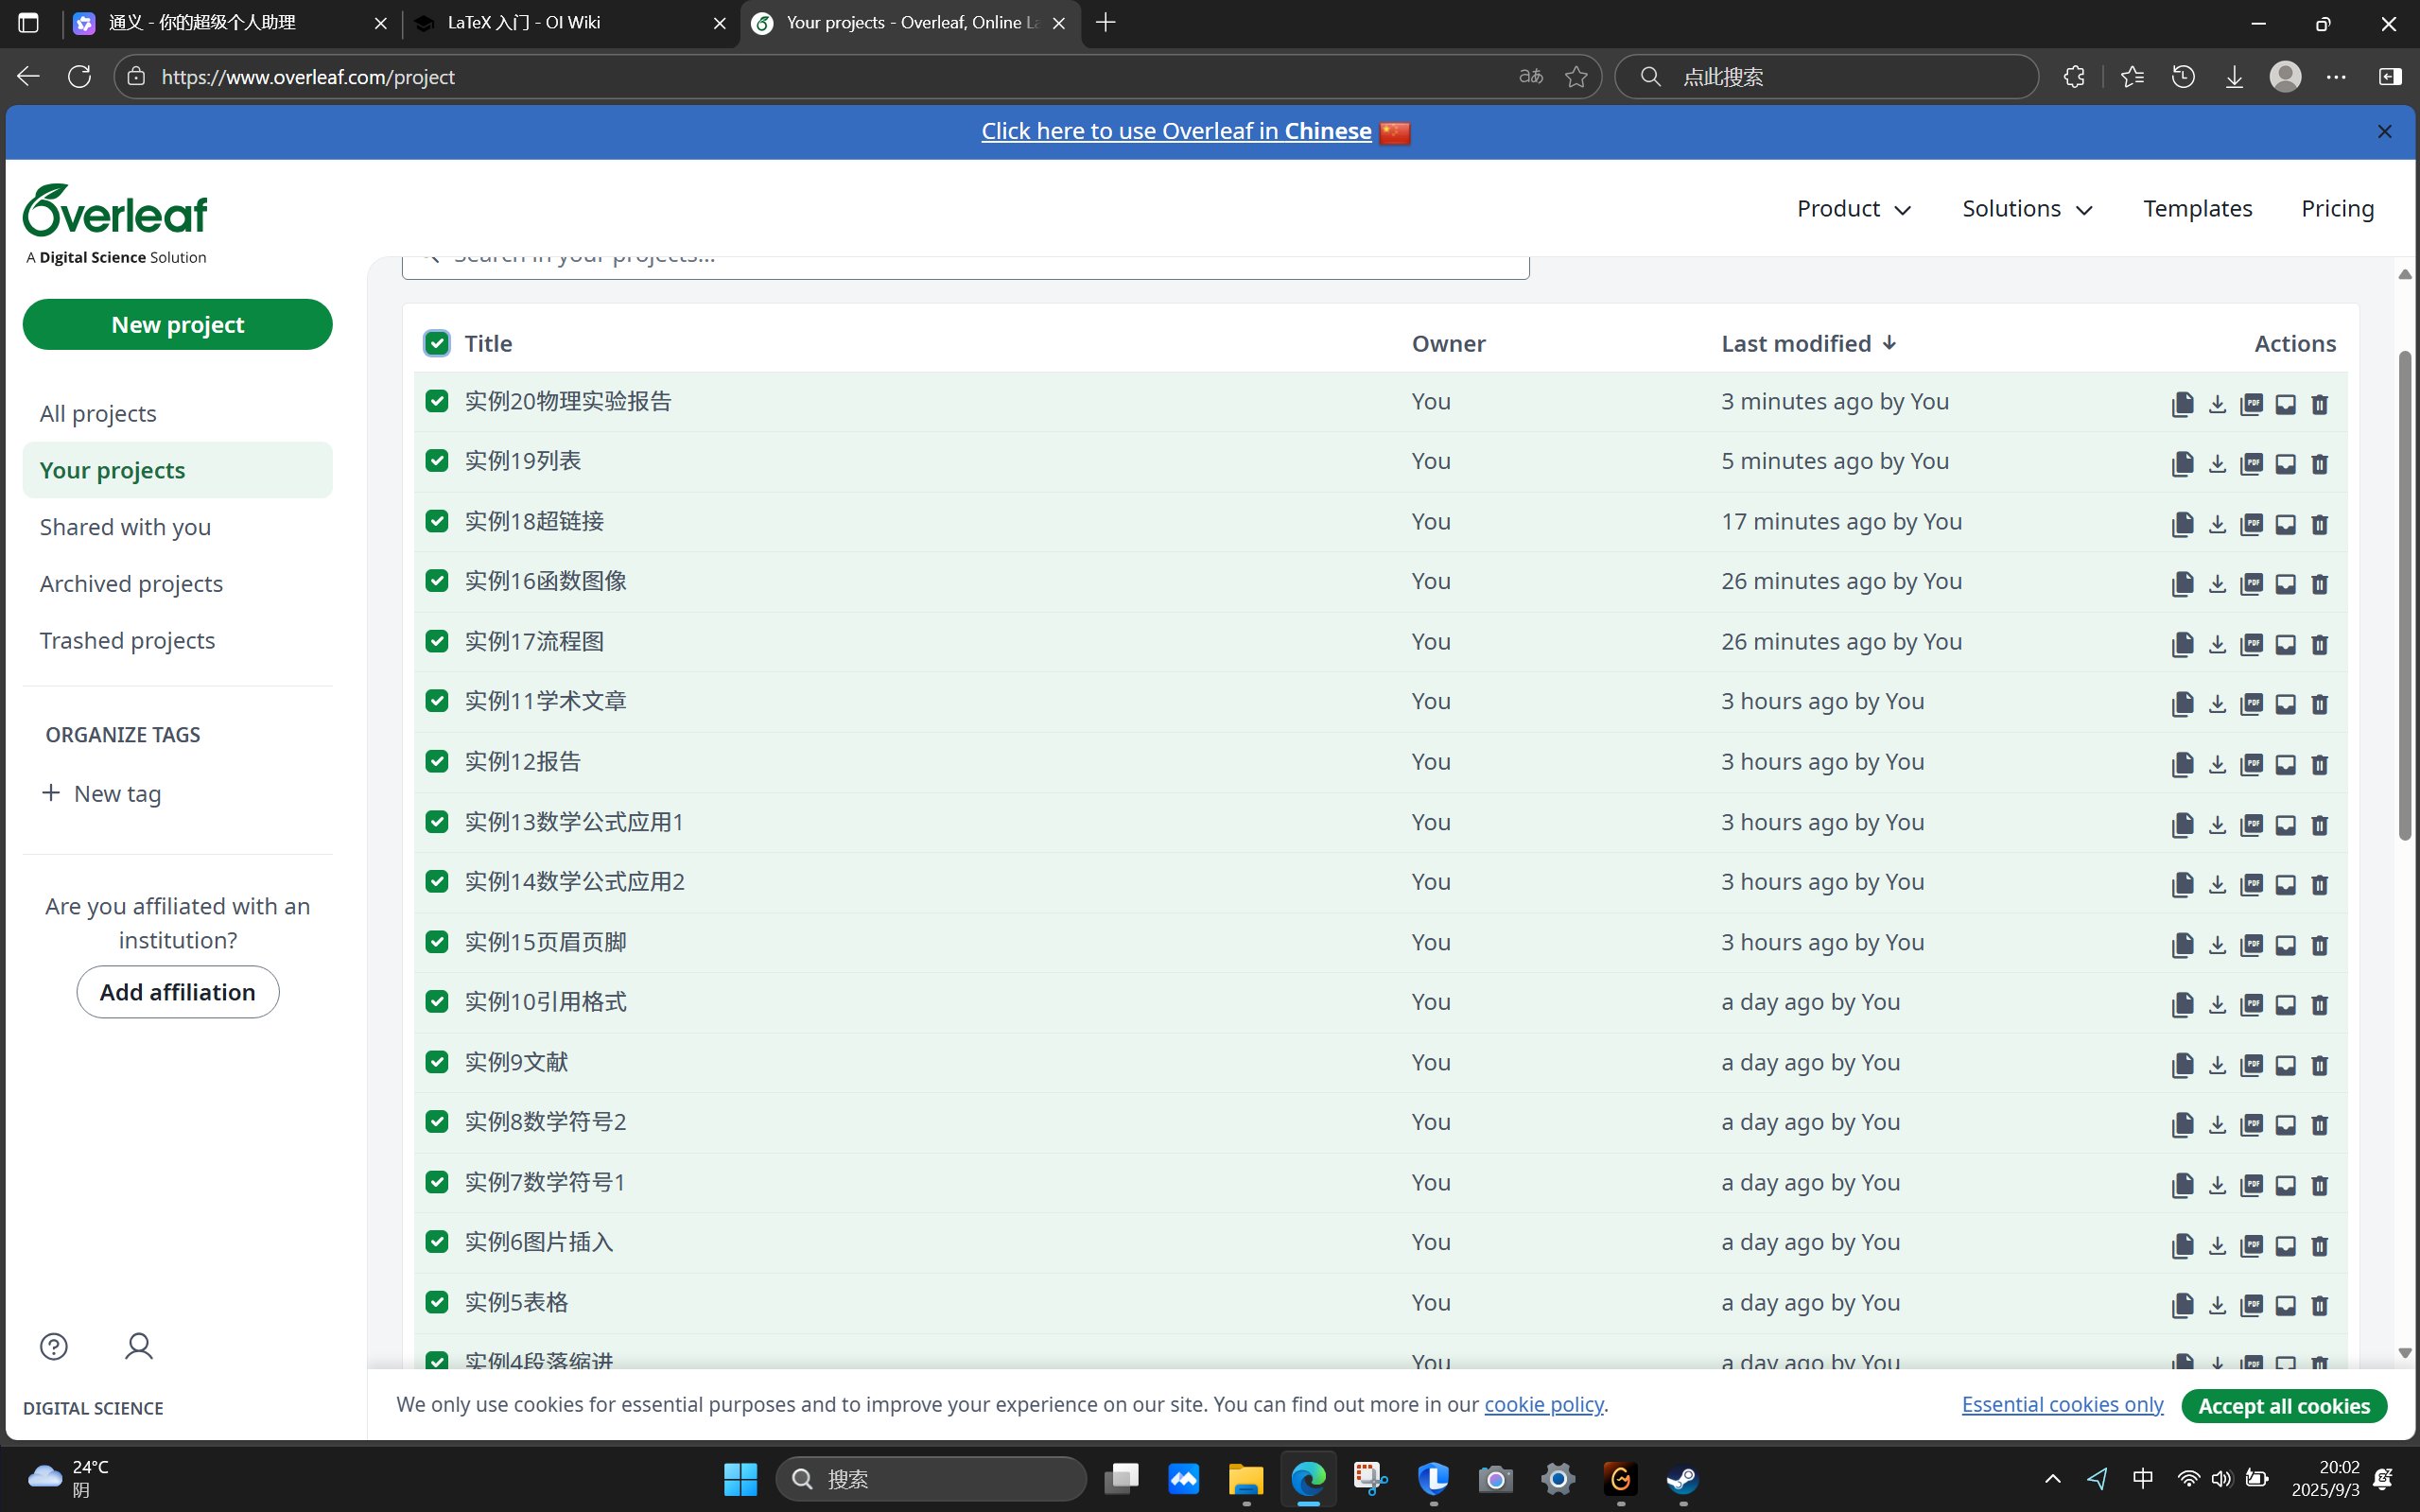
\includegraphics[width=0.8\textwidth]{20个latex实例.png}%0.8倍文本宽度
        \caption{完成了20个latex实例}
        \label{fig:实例}
\end{figure}

\section*{六、解题感悟}
通过本次实验,我深入了解了 LaTeX 文档的编写流程和 Git 版本控制的基本操作。具体收获如下:
\begin{itemize}
    \item LaTeX 是一种非常强大的排版工具,特别适合学术论文和技术文档的撰写。
    \item Git 提供了高效的版本控制功能,能够帮助开发者更好地管理代码或文档的变更历史。通过前10个实例的动手实践,我熟悉了 \texttt{init}, \texttt{add}, \texttt{commit}, \texttt{push}, \texttt{pull} 等核心命令,理解了“工作区-暂存区-仓库”的工作流,为未来的团队协作和项目管理打下了坚实基础。
\end{itemize}

\section*{七、GitHub链接}
本次实验的全部代码、文档及20个latex实例可以在 GitHub 上找到:\url{https://github.com/ouc-lhy/for-lesson/tree/master/lesson1} 或者直接点击 \href{https://github.com/ouc-lhy/for-lesson/tree/master/lesson1}{这里} 查看。

\end{document}